\documentclass[12pt]{article}
%\usepackage[utf8]{inputenc}
%\documentclass[UTF8]{ctexart}
%\usepackage[UTF8, heading = false, scheme = plain]{ctex}
\usepackage{geometry}
%geometry{a4paper,scale=0.9}
\geometry{a4paper,left=1cm,right=1cm,top=1cm,bottom=2cm}
\usepackage{amsfonts}
\usepackage{color}
\usepackage{url}
%\usepackage{biblatex}
\usepackage{amsmath}
\usepackage{amssymb}
\usepackage{latexsym}
\usepackage{listings}
\usepackage[usenames,dvipsnames]{xcolor}
\usepackage{cite}
%\addbibresource{ref.bib}
%\bibliography{ref.bib}
\usepackage{caption}
\usepackage{graphicx, subfig}
\usepackage{float}
%\usepackage[fontset=ubuntu]{ctex}
%\usepackage{fontspec}
\usepackage{xeCJK}
%\usepackage[colorlinks,
%anchorcolor=black,
%citecolor=black]{hyperref}
%\setmainfont{SimSun}
\usepackage[section]{placeins}
\usepackage{enumitem}
\usepackage{framed}
\usepackage[framemethod=TikZ]{mdframed}
\usepackage{indentfirst}
\usepackage{setspace}%使用间距宏包
\linespread{1.5}
\definecolor{mygreen}{rgb}{0,0.6,0}
\definecolor{mygray}{rgb}{0.5,0.5,0.5}
\definecolor{mybgray}{rgb}{0.95,0.95,0.95}
\definecolor{mymauve}{rgb}{0.58,0,0.82}
\lstset{
 backgroundcolor=\color{mybgray}, 
 basicstyle = \footnotesize,       
 breakatwhitespace = false,        
 breaklines = true,                 
 captionpos = b,                    
 commentstyle = \color{mygreen}\bfseries,
 extendedchars = false,             
 frame =shadowbox, 
 framerule=0.5pt,
 keepspaces=true,
 keywordstyle=\color{blue}\bfseries, % keyword style
 language = C++,                     % the language of code
 otherkeywords={string}, 
 numbers=left, 
 numbersep=5pt,
 numberstyle=\tiny\color{mygray},
 rulecolor=\color{black},         
 showspaces=false,  
 showstringspaces=false, 
 showtabs=false,    
 stepnumber=1,         
 stringstyle=\color{mymauve},        % string literal style
 tabsize=2,          
 title=\lstname                      
}

\title{数据结构}
\author{leolinuxer}
%\date{June 2020}

\begin{document}
%\setlength{\parindent}{0pt}
\maketitle
\tableofcontents

\section{二叉堆和优先级}
\url{https://github.com/labuladong/fucking-algorithm/blob/master/%E6%95%B0%E6%8D%AE%E7%BB%93%E6%9E%84%E7%B3%BB%E5%88%97/%E4%BA%8C%E5%8F%89%E5%A0%86%E8%AF%A6%E8%A7%A3%E5%AE%9E%E7%8E%B0%E4%BC%98%E5%85%88%E7%BA%A7%E9%98%9F%E5%88%97.md}

二叉堆(Binary Heap)没什么神秘,性质比二叉搜索树 BST 还简单。其主要操作就两个,sink(下沉)和 swim(上浮),用以维护二叉堆的性质。其主要应用有两个,首先是一种排序方法「堆排序」,第二是一种很有用的数据结构「优先级队列」。

本文就以实现优先级队列(Priority Queue)为例,通过图片和人类的语言来描述一下二叉堆怎么运作的。

\subsection{二叉堆概览}
首先,二叉堆和二叉树有啥关系呢,为什么人们总数把二叉堆画成一棵二叉树?因为,\textbf{二叉堆其实就是一种特殊的二叉树(完全二叉树),只不过存储在数组里}。一般的链表二叉树,我们操作节点的指针,而在数组里,我们把数组索引作为指针:
\begin{lstlisting}
// 父节点的索引
int parent(int root) {
    return root / 2;
}
// 左孩子的索引
int left(int root) {
    return root * 2;
}
// 右孩子的索引
int right(int root) {
    return root * 2 + 1;
}
\end{lstlisting}

画个图你立即就能理解了,注意数组的第一个索引 0 空着不用,
\begin{figure}[H]
    \centering
    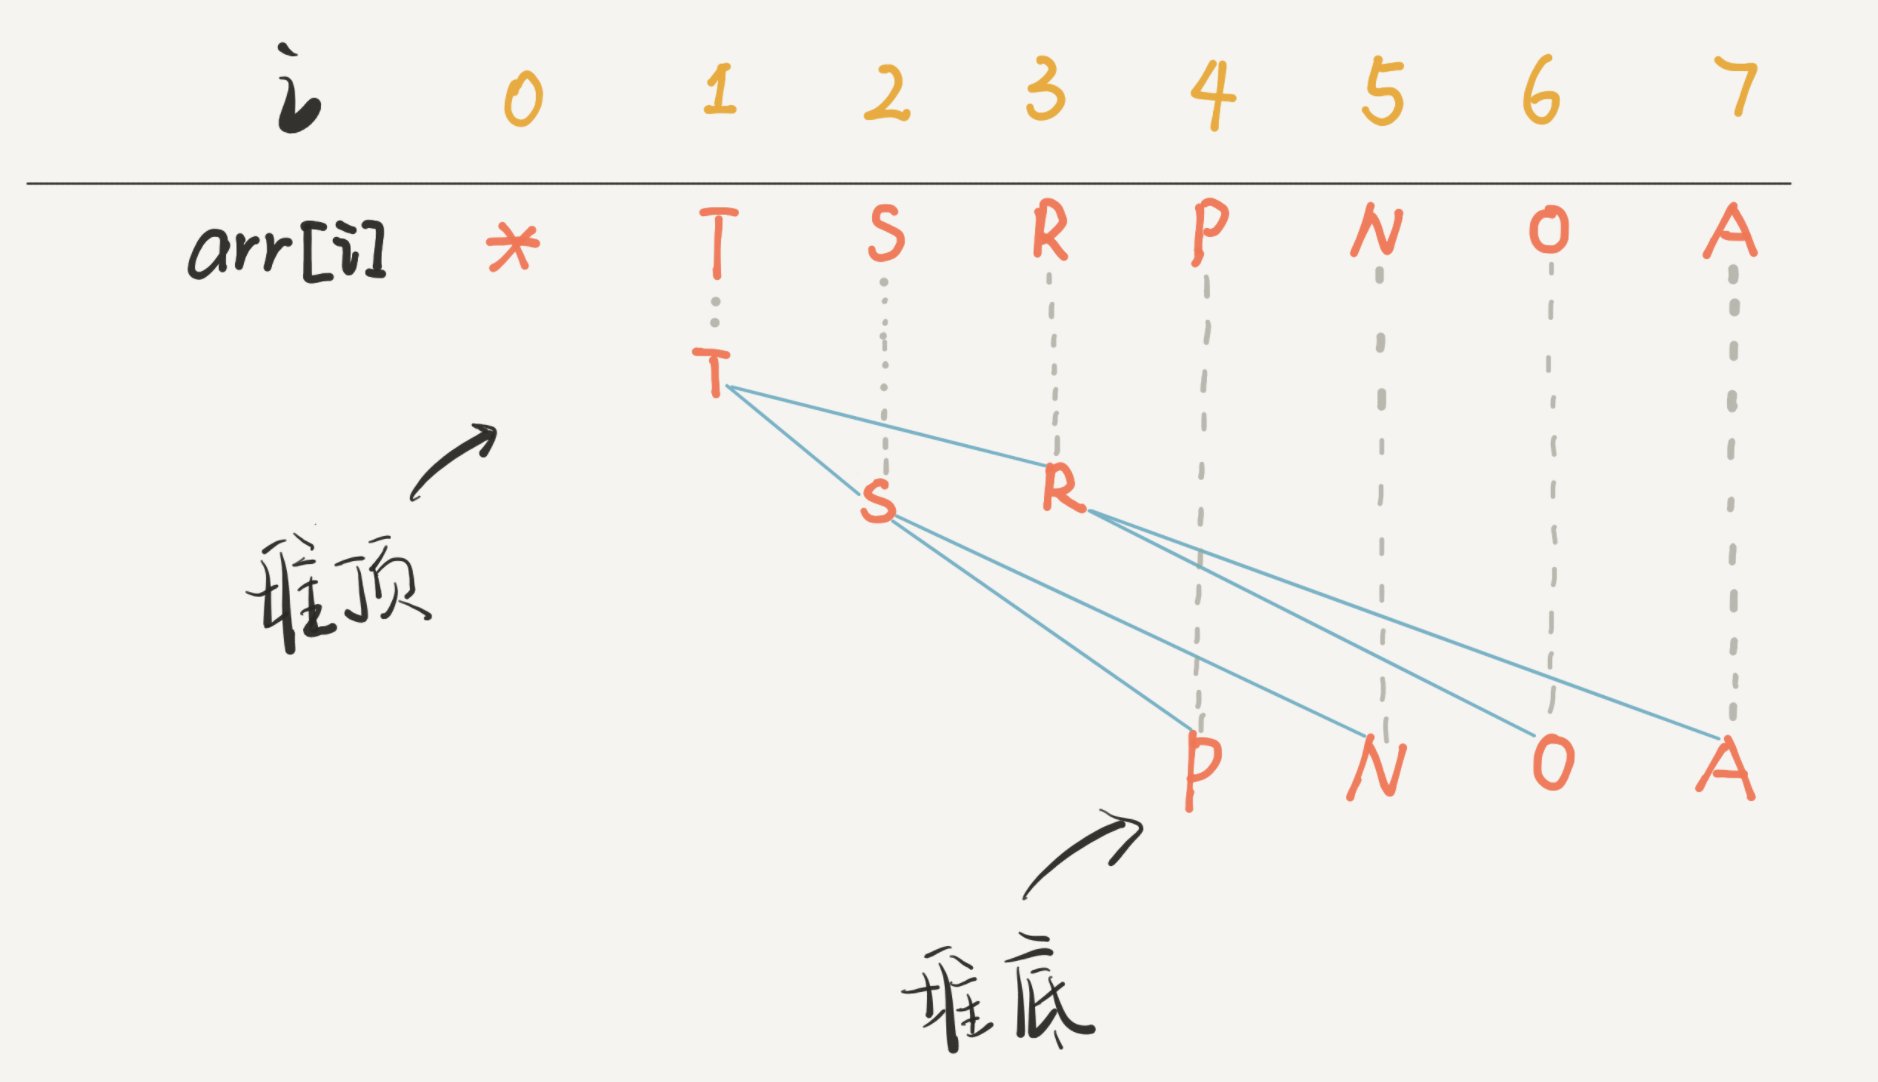
\includegraphics[width=.6\textwidth]{fig/Binary_Heap_1.png}
\end{figure}
PS:因为数组索引是数组,为了方便区分,将字符作为数组元素。

你看到了,把 arr[1] 作为整棵树的根的话,每个节点的父节点和左右孩子的索引都可以通过简单的运算得到,这就是二叉堆设计的一个巧妙之处。为了方便讲解,下面都会画的图都是二叉树结构,相信你能把树和数组对应起来。

二叉堆还分为最大堆和最小堆。\textbf{最大堆的性质是:每个节点都大于等于它的两个子节点。类似的,最小堆的性质是:每个节点都小于等于它的子节点}。

两种堆核心思路都是一样的,本文以最大堆为例讲解。

对于一个最大堆,根据其性质,显然堆顶,也就是 arr[1] 一定是所有元素中最大的元素。

\subsection{优先级队列概览}
优先级队列这种数据结构有一个很有用的功能,你插入或者删除元素的时候,元素会自动排序,这底层的原理就是二叉堆的操作。

数据结构的功能无非增删查该,优先级队列有两个主要 API,分别是 insert 插入一个元素和 delMax 删除最大元素(如果底层用最小堆,那么就是 delMin)。

下面我们实现一个简化的优先级队列,先看下代码框架:

PS:为了清晰起见,这里用到 Java 的泛型,Key 可以是任何一种可比较大小的数据类型,你可以认为它是 int、char 等。
\begin{lstlisting}
public class MaxPQ
    <Key extends Comparable<Key>> {
    // 存储元素的数组
    private Key[] pq;
    // 当前 Priority Queue 中的元素个数
    private int N = 0;

    public MaxPQ(int cap) {
        // 索引 0 不用,所以多分配一个空间
        pq = (Key[]) new Comparable[cap + 1];
    }

    /* 返回当前队列中最大元素 */
    public Key max() {
        return pq[1];
    }

    /* 插入元素 e */
    public void insert(Key e) {...}

    /* 删除并返回当前队列中最大元素 */
    public Key delMax() {...}

    /* 上浮第 k 个元素,以维护最大堆性质 */
    private void swim(int k) {...}

    /* 下沉第 k 个元素,以维护最大堆性质 */
    private void sink(int k) {...}

    /* 交换数组的两个元素 */
    private void exch(int i, int j) {
        Key temp = pq[i];
        pq[i] = pq[j];
        pq[j] = temp;
    }

    /* pq[i] 是否比 pq[j] 小? */
    private boolean less(int i, int j) {
        return pq[i].compareTo(pq[j]) < 0;
    }

    /* 还有 left, right, parent 三个方法 */
}
\end{lstlisting}

空出来的四个方法是二叉堆和优先级队列的奥妙所在,下面用图文来逐个理解。

\subsection{实现 swim 和 sink}
为什么要有上浮 swim 和下沉 sink 的操作呢?为了维护堆结构。

我们要讲的是最大堆,每个节点都比它的两个子节点大,但是在插入元素和删除元素时,难免破坏堆的性质,这就需要通过这两个操作来恢复堆的性质了。

对于最大堆,会破坏堆性质的有有两种情况:
\begin{itemize}
\setlength{\itemsep}{0pt}
\setlength{\parsep}{0pt}
\setlength{\parskip}{0pt}
    \item 如果某个节点 A 比它的子节点(中的一个)小,那么 A 就不配做父节点,应该下去,下面那个更大的节点上来做父节点,这就是对 A 进行下沉;
    \item 如果某个节点 A 比它的父节点大,那么 A 不应该做子节点,应该把父节点换下来,自己去做父节点,这就是对 A 的上浮;
\end{itemize}

当然,错位的节点 A 可能要上浮(或下沉)很多次,才能到达正确的位置,恢复堆的性质。所以代码中肯定有一个 while 循环

细心的读者也许会问,这两个操作不是互逆吗,所以上浮的操作一定能用下沉来完成,为什么我还要费劲写两个方法?是的,操作是互逆等价的,但是最终我们的操作只会在堆底和堆顶进行(等会讲原因),显然堆底的「错位」元素需要上浮,堆顶的「错位」元素需要下沉。

\subsubsection{上浮的代码实现}
\begin{lstlisting}
private void swim(int k) {
    // 如果浮到堆顶,就不能再上浮了
    while (k > 1 && less(parent(k), k)) {
        // 如果第 k 个元素比上层大
        // 将 k 换上去
        exch(parent(k), k);
        k = parent(k);
    }
}
\end{lstlisting}

\subsubsection{下沉的代码实现}
下沉比上浮略微复杂一点,因为上浮某个节点 A,只需要 A 和其父节点比较大小即可;但是下沉某个节点 A,需要 A 和其两个子节点比较大小,如果 A 不是最大的就需要调整位置,要把较大的那个子节点和 A 交换。
\begin{lstlisting}
private void sink(int k) {
    // 如果沉到堆底,就沉不下去了
    while (left(k) <= N) {
        // 先假设左边节点较大
        int older = left(k);
        // 如果右边节点存在,比一下大小
        if (right(k) <= N && less(older, right(k)))
            older = right(k);
        // 结点 k 比俩孩子都大,就不必下沉了
        if (less(older, k)) break;
        // 否则,不符合最大堆的结构,下沉 k 结点
        exch(k, older);
        k = older;
    }
}
\end{lstlisting}

至此,二叉堆的主要操作就讲完了,一点都不难吧,代码加起来也就十行。明白了 sink 和 swim 的行为,下面就可以实现优先级队列了。

\subsection{实现 delMax 和 insert}
这两个方法就是建立在 swim 和 sink 上的。

\textbf{insert 方法先把要插入的元素添加到堆底的最后,然后让其上浮到正确位置}。
\begin{lstlisting}
public void insert(Key e) {
    N++;
    // 先把新元素加到最后
    pq[N] = e;
    // 然后让它上浮到正确的位置
    swim(N);
}
\end{lstlisting}

\textbf{delMax 方法先把堆顶元素 A 和堆底最后的元素 B 对调,然后删除 A,最后让 B 下沉到正确位置}。
\begin{lstlisting}
public Key delMax() {
    // 最大堆的堆顶就是最大元素
    Key max = pq[1];
    // 把这个最大元素换到最后,删除之
    exch(1, N);
    pq[N] = null;
    N--;
    // 让 pq[1] 下沉到正确位置
    sink(1);
    return max;
}
\end{lstlisting}

至此,一个优先级队列就实现了,插入和删除元素的时间复杂度为 $O(logK)$,$K$ 为当前二叉堆(优先级队列)中的元素总数。因为我们时间复杂度主要花费在 sink 或者 swim 上,而不管上浮还是下沉,最多也就树(堆)的高度,也就是 log 级别。

\subsection{总结}
二叉堆就是一种完全二叉树,所以适合存储在数组中,而且二叉堆拥有一些特殊性质。

二叉堆的操作很简单,主要就是上浮和下沉,来维护堆的性质(堆有序),核心代码也就十行。

优先级队列是基于二叉堆实现的,主要操作是插入和删除。插入是先插到最后,然后上浮到正确位置;删除是调换位置后再删除,然后下沉到正确位置。核心代码也就十行。

\section{LRU算法详解——哈希链表}
\url{https://github.com/labuladong/fucking-algorithm/blob/master/%E9%AB%98%E9%A2%91%E9%9D%A2%E8%AF%95%E7%B3%BB%E5%88%97/LRU%E7%AE%97%E6%B3%95.md}
\subsection{什么是 LRU 算法}
LRU 算法就是一种缓存淘汰策略:计算机的缓存容量有限,如果缓存满了就要删除一些内容,给新内容腾位置。但问题是,删除哪些内容呢?我们肯定希望删掉哪些没什么用的缓存,而把有用的数据继续留在缓存里,方便之后继续使用。那么,什么样的数据,我们判定为「有用的」的数据呢?

LRU 缓存淘汰算法就是一种常用策略。LRU 的全称是 Least Recently Used,也就是说我们认为最近使用过的数据应该是是「有用的」,很久都没用过的数据应该是无用的,内存满了就优先删那些很久没用过的数据。

当然还有其他缓存淘汰策略,比如不要按访问的时序来淘汰,而是按访问频率(LFU 策略)来淘汰等等,各有应用场景。本文讲解 LRU 算法策略。

\subsection{LRU 算法描述}
LRU 算法实际上是让你设计数据结构:首先要接收一个 capacity 参数作为缓存的最大容量,然后实现两个 API,一个是 put(key, val) 方法存入键值对,另一个是 get(key) 方法获取 key 对应的 val,如果 key 不存在则返回 -1。

注意哦,get 和 put 方法必须都是 $O(1)$ 的时间复杂度,我们举个具体例子来看看 LRU 算法怎么工作。
\begin{lstlisting}
/* 缓存容量为 2 */
LRUCache cache = new LRUCache(2);
// 你可以把 cache 理解成一个队列
// 假设左边是队头,右边是队尾
// 最近使用的排在队头,久未使用的排在队尾
// 圆括号表示键值对 (key, val)

cache.put(1, 1);
// cache = [(1, 1)]
cache.put(2, 2);
// cache = [(2, 2), (1, 1)]
cache.get(1);       // 返回 1
// cache = [(1, 1), (2, 2)]
// 解释:因为最近访问了键 1,所以提前至队头
// 返回键 1 对应的值 1
cache.put(3, 3);
// cache = [(3, 3), (1, 1)]
// 解释:缓存容量已满,需要删除内容空出位置
// 优先删除久未使用的数据,也就是队尾的数据
// 然后把新的数据插入队头
cache.get(2);       // 返回 -1 (未找到)
// cache = [(3, 3), (1, 1)]
// 解释:cache 中不存在键为 2 的数据
cache.put(1, 4);    
// cache = [(1, 4), (3, 3)]
// 解释:键 1 已存在,把原始值 1 覆盖为 4
// 不要忘了也要将键值对提前到队头
\end{lstlisting}

\subsection{LRU 算法设计}
分析上面的操作过程,要让 put 和 get 方法的时间复杂度为 O(1),我们可以总结出 cache 这个数据结构必要的条件:查找快,插入快,删除快,有顺序之分。

因为显然 cache 必须有顺序之分,以区分最近使用的和久未使用的数据;而且我们要在 cache 中查找键是否已存在;如果容量满了要删除最后一个数据;每次访问还要把数据插入到队头。

那么,什么数据结构同时符合上述条件呢?哈希表查找快,但是数据无固定顺序;链表有顺序之分,插入删除快,但是查找慢。所以结合一下,形成一种新的数据结构:\textbf{哈希链表}。

LRU 缓存算法的核心数据结构就是哈希链表,双向链表和哈希表的结合体。这个数据结构长这样:
\begin{figure}[H]
    \centering
    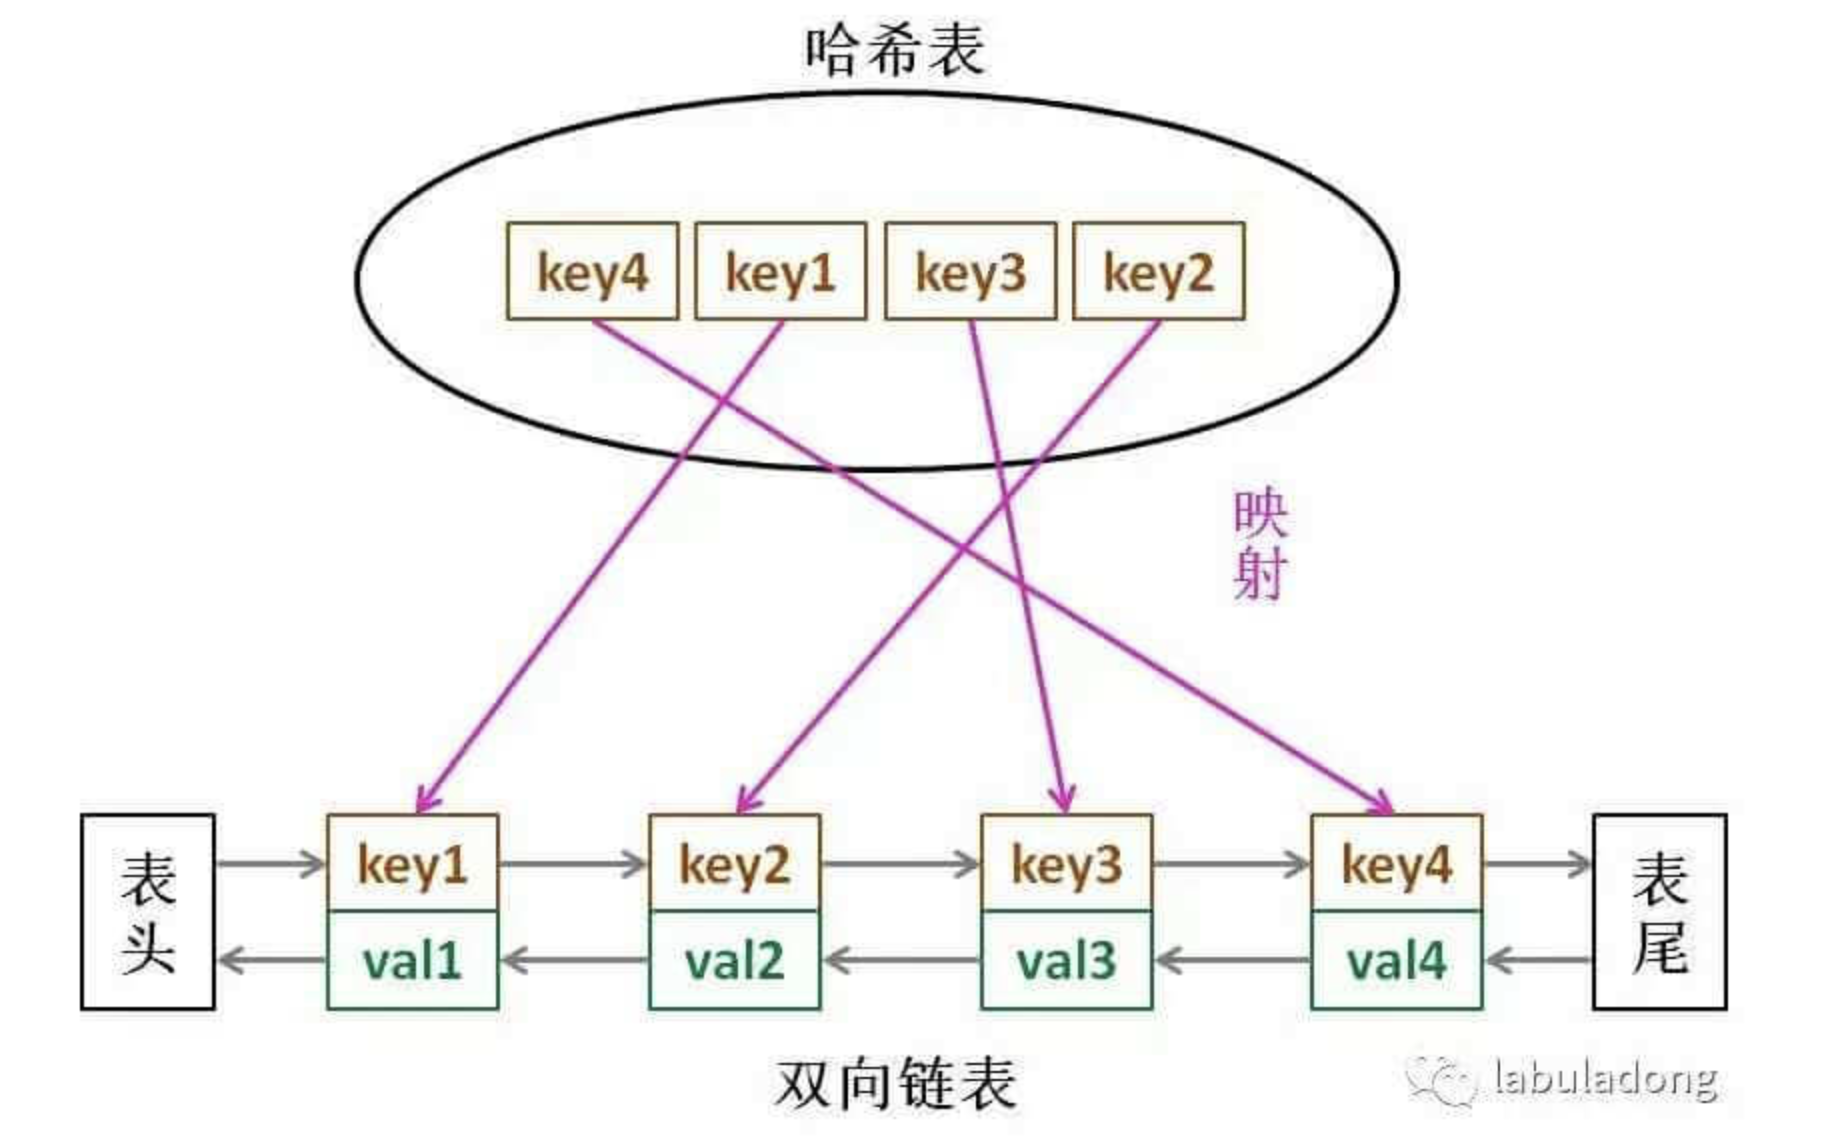
\includegraphics[width=1\textwidth]{fig/LRU_1.png}
\end{figure}

思想很简单,就是借助哈希表赋予了链表快速查找的特性嘛:可以快速查找某个 key 是否存在缓存(链表)中,同时可以快速删除、添加节点。回想刚才的例子,这种数据结构是不是完美解决了 LRU 缓存的需求?

也许读者会问,为什么要是双向链表,单链表行不行?另外,既然哈希表中已经存了 key,为什么链表中还要存键值对呢,只存值不就行了?想的时候都是问题,只有做的时候才有答案。这样设计的原因,必须等我们亲自实现 LRU 算法之后才能理解,所以我们开始看代码吧~

\subsection{代码实现}
首先,我们把双链表的节点类写出来,为了简化,key 和 val 都认为是 int 类型:
\begin{lstlisting}
class Node {
    public int key, val;
    public Node next, prev;
    public Node(int k, int v) {
        this.key = k;
        this.val = v;
    }
}
\end{lstlisting}

然后依靠我们的 Node 类型构建一个双链表,实现几个需要的 API(这些操作的时间复杂度均为 $O(1)$):
\begin{lstlisting}
class DoubleList {  
    // 在链表头部添加节点 x,时间 O(1)
    public void addFirst(Node x);

    // 删除链表中的 x 节点(x 一定存在)
    // 由于是双链表且给的是目标 Node 节点,时间 O(1)
    public void remove(Node x);
    
    // 删除链表中最后一个节点,并返回该节点,时间 O(1)
    public Node removeLast();
    
    // 返回链表长度,时间 O(1)
    public int size();
}
\end{lstlisting}
PS:这就是普通双向链表的实现,为了让读者集中精力理解 LRU 算法的逻辑,就省略链表的具体代码。

到这里就能回答刚才“为什么必须要用双向链表”的问题了,因为我们需要删除操作。删除一个节点不光要得到该节点本身的指针,也需要操作其前驱节点的指针,而双向链表才能支持直接查找前驱,保证操作的时间复杂度 $O(1)$。

有了双向链表的实现,我们只需要在 LRU 算法中把它和哈希表结合起来即可。我们先把逻辑理清楚:
\begin{lstlisting}
// key 映射到 Node(key, val)
HashMap<Integer, Node> map;
// Node(k1, v1) <-> Node(k2, v2)...
DoubleList cache;

int get(int key) {
    if (key 不存在) {
        return -1;
    } else {        
        将数据 (key, val) 提到开头;
        return val;
    }
}

void put(int key, int val) {
    Node x = new Node(key, val);
    if (key 已存在) {
        把旧的数据删除;
        将新节点 x 插入到开头;
    } else {
        if (cache 已满) {
            删除链表的最后一个数据腾位置;
            删除 map 中映射到该数据的键;
        } 
        将新节点 x 插入到开头;
        map 中新建 key 对新节点 x 的映射;
    }
}
\end{lstlisting}

如果能够看懂上述逻辑,翻译成代码就很容易理解了:
\begin{lstlisting}
class LRUCache {
    // key -> Node(key, val)
    private HashMap<Integer, Node> map;
    // Node(k1, v1) <-> Node(k2, v2)...
    private DoubleList cache;
    // 最大容量
    private int cap;
    
    public LRUCache(int capacity) {
        this.cap = capacity;
        map = new HashMap<>();
        cache = new DoubleList();
    }
    
    public int get(int key) {
        if (!map.containsKey(key))
            return -1;
        int val = map.get(key).val;
        // 利用 put 方法把该数据提前
        put(key, val);
        return val;
    }
    
    public void put(int key, int val) {
        // 先把新节点 x 做出来
        Node x = new Node(key, val);
        
        if (map.containsKey(key)) {
            // 删除旧的节点,新的插到头部
            cache.remove(map.get(key));
            cache.addFirst(x);
            // 更新 map 中对应的数据
            map.put(key, x);
        } else {
            if (cap == cache.size()) {
                // 删除链表最后一个数据
                Node last = cache.removeLast();
                map.remove(last.key);
            }
            // 直接添加到头部
            cache.addFirst(x);
            map.put(key, x);
        }
    }
}
\end{lstlisting}

这里就能回答之前的问答题“为什么要在链表中同时存储 key 和 val,而不是只存储 val”,注意这段代码:
\begin{lstlisting}
if (cap == cache.size()) {
    // 删除链表最后一个数据
    Node last = cache.removeLast();
    map.remove(last.key);
}
\end{lstlisting}
当缓存容量已满,我们不仅仅要删除最后一个 Node 节点,还要把 map 中映射到该节点的 key 同时删除,而这个 key 只能由 Node 得到。如果 Node 结构中只存储 val,那么我们就无法得知 key 是什么,就无法删除 map 中的键,造成错误。

至此,你应该已经掌握 LRU 算法的思想和实现了,很容易犯错的一点是:处理链表节点的同时不要忘了更新哈希表中对节点的映射。

\section{二叉搜索树}
\url{https://github.com/labuladong/fucking-algorithm/blob/master/%E6%95%B0%E6%8D%AE%E7%BB%93%E6%9E%84%E7%B3%BB%E5%88%97/%E4%BA%8C%E5%8F%89%E6%90%9C%E7%B4%A2%E6%A0%91%E6%93%8D%E4%BD%9C%E9%9B%86%E9%94%A6.md}
\subsection{总体思路}
二叉树算法的设计的总路线:明确一个节点要做的事情,然后剩下的事抛给框架。
\begin{lstlisting}
void traverse(TreeNode root) {
    // root 需要做什么?在这做。
    // 其他的不用 root 操心,抛给框架
    traverse(root.left);
    traverse(root.right);
}
\end{lstlisting}

举两个简单的例子体会一下这个思路,热热身。

1. 如何把二叉树所有的节点中的值加一?
\begin{lstlisting}
void plusOne(TreeNode root) {
    if (root == null) return;
    root.val += 1;

    plusOne(root.left);
    plusOne(root.right);
}
\end{lstlisting}

如何判断两棵二叉树是否完全相同?
\begin{lstlisting}
boolean isSameTree(TreeNode root1, TreeNode root2) {
    // 都为空的话,显然相同
    if (root1 == null && root2 == null) return true;
    // 一个为空,一个非空,显然不同
    if (root1 == null || root2 == null) return false;
    // 两个都非空,但 val 不一样也不行
    if (root1.val != root2.val) return false;

    // root1 和 root2 该比的都比完了
    return isSameTree(root1.left, root2.left)
        && isSameTree(root1.right, root2.right);
    // 注意这里的 && 条件,必须所有的子节点都返回 true,最终才会返回 true
}
\end{lstlisting}

\subsection{二叉搜索树}
二叉搜索树(Binary Search Tree,简称 BST)是一种很常用的的二叉树。它的定义是:一个二叉树中,任意节点的值要大于等于左子树所有节点的值,且要小于等于右边子树的所有节点的值。

如下就是一个符合定义的 BST:
\begin{figure}[H]
    \centering
    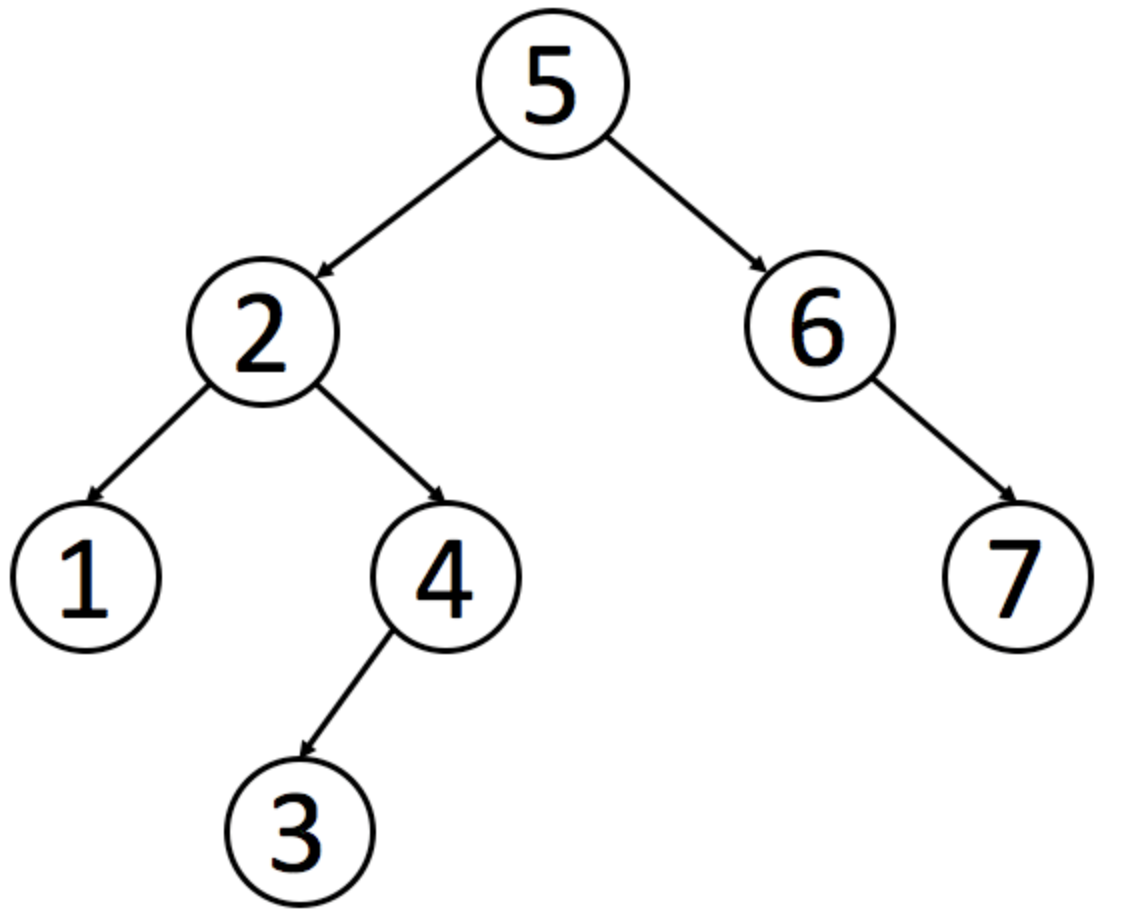
\includegraphics[width=.3\textwidth]{fig/BST_1.png}
\end{figure}

下面实现 BST 的基础操作:判断 BST 的合法性、增、删、查。其中“删”和“判断合法性”略微复杂。
\subsubsection{判断 BST 的合法性}
这里是有坑的哦,我们按照刚才的思路,每个节点自己要做的事不就是比较自己和左右孩子吗?看起来应该这样写代码:
\begin{lstlisting}
boolean isValidBST(TreeNode root) {
    if (root == null) return true;
    if (root.left != null && root.val <= root.left.val) return false;
    if (root.right != null && root.val >= root.right.val) return false;

    return isValidBST(root.left)
        && isValidBST(root.right);
}
\end{lstlisting}

但是这个算法出现了错误,BST 的每个节点应该要小于右边子树的\textbf{所有}节点,下面这个二叉树显然不是 BST,但是我们的算法会把它判定为 BST。
\begin{figure}[H]
    \centering
    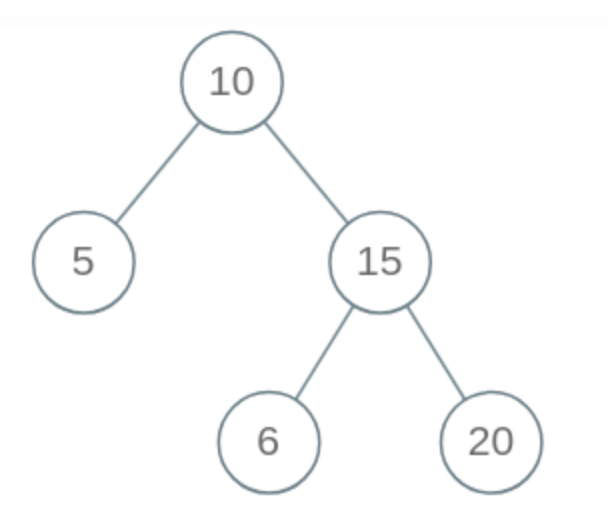
\includegraphics[width=.3\textwidth]{fig/BST_2.png}
\end{figure}
出现错误,不要慌张,框架没有错,一定是某个细节问题没注意到。我们重新看一下 BST 的定义,root 需要做的不只是和左右子节点比较,而是要整个左子树和右子树所有节点比较。怎么办,鞭长莫及啊!

这种情况,我们可以使用辅助函数,增加函数参数列表,在参数中携带额外信息,请看正确的代码:
\begin{lstlisting}
boolean isValidBST(TreeNode root) {
    return isValidBST(root, null, null);
}

boolean isValidBST(TreeNode root, TreeNode min, TreeNode max) {
    if (root == null) return true;
    if (min != null && root.val <= min.val) return false;
    if (max != null && root.val >= max.val) return false;
    return isValidBST(root.left, min, root) 
        && isValidBST(root.right, root, max);
}
\end{lstlisting}

\subsubsection{在 BST 中查找一个数是否存在}
根据我们的指导思想,可以这样写代码:
\begin{lstlisting}
boolean isInBST(TreeNode root, int target) {
    if (root == null) return false;
    if (root.val == target) return true;

    return isInBST(root.left, target)
        || isInBST(root.right, target);
}
\end{lstlisting}

这样写完全正确,充分证明了你的框架性思维已经养成。现在你可以考虑一点细节问题了:如何充分利用信息,把 BST 这个“左小右大”的特性用上?

很简单,其实不需要递归地搜索两边,类似二分查找思想,根据 target 和 root.val 的大小比较,就能排除一边。我们把上面的思路稍稍改动:

\begin{lstlisting}
boolean isInBST(TreeNode root, int target) {
    if (root == null) return false;
    if (root.val == target)
        return true;
    if (root.val < target) 
        return isInBST(root.right, target);
    if (root.val > target)
        return isInBST(root.left, target);
    // root 该做的事做完了,顺带把框架也完成了,妙
}
\end{lstlisting}

于是,我们对原始框架进行改造,抽象出一套针对 BST 的遍历框架:
\begin{lstlisting}
void BST(TreeNode root, int target) {
    if (root.val == target)
        // 找到目标,做点什么
    if (root.val < target) 
        BST(root.right, target);
    if (root.val > target)
        BST(root.left, target);
}
\end{lstlisting}

\subsubsection{在 BST 中插入一个数}
对数据结构的操作无非遍历 + 访问,遍历就是“找”,访问就是“改”。具体到这个问题,插入一个数,就是先找到插入位置,然后进行插入操作。

上一个问题,我们总结了 BST 中的遍历框架,就是“找”的问题。直接套框架,加上“改”的操作即可。\textbf{一旦涉及“改”,函数就要返回 TreeNode 类型,并且对递归调用的返回值进行接收}。
\begin{lstlisting}
TreeNode insertIntoBST(TreeNode root, int val) {
    // 找到空位置插入新节点
    if (root == null) return new TreeNode(val);
    // if (root.val == val)
    //     BST 中一般不会插入已存在元素
    if (root.val < val) 
        root.right = insertIntoBST(root.right, val);
    if (root.val > val) 
        root.left = insertIntoBST(root.left, val);
    return root;
}
\end{lstlisting}
\begin{framed}
理解:BST 最终都是在叶子节点插入数的,这样的插入操作最简单,但是会破坏 BST 的平衡性
\end{framed}

\subsubsection{在 BST 中删除一个数}
这个问题稍微复杂,不过你有框架指导,难不住你。跟插入操作类似,先“找”再“改”,先把框架写出来再说:
\begin{lstlisting}
TreeNode deleteNode(TreeNode root, int key) {
    if (root.val == key) {
        // 找到啦,进行删除
    } else if (root.val > key) {
        root.left = deleteNode(root.left, key);
    } else if (root.val < key) {
        root.right = deleteNode(root.right, key);
    }
    return root;
}
\end{lstlisting}

找到目标节点了,比方说是节点 A,如何删除这个节点,这是难点。因为删除节点的同时不能破坏 BST 的性质。有三种情况,用图片来说明。

情况 1:A 恰好是末端节点,两个子节点都为空,那么它可以当场去世了。
\begin{figure}[H]
    \centering
    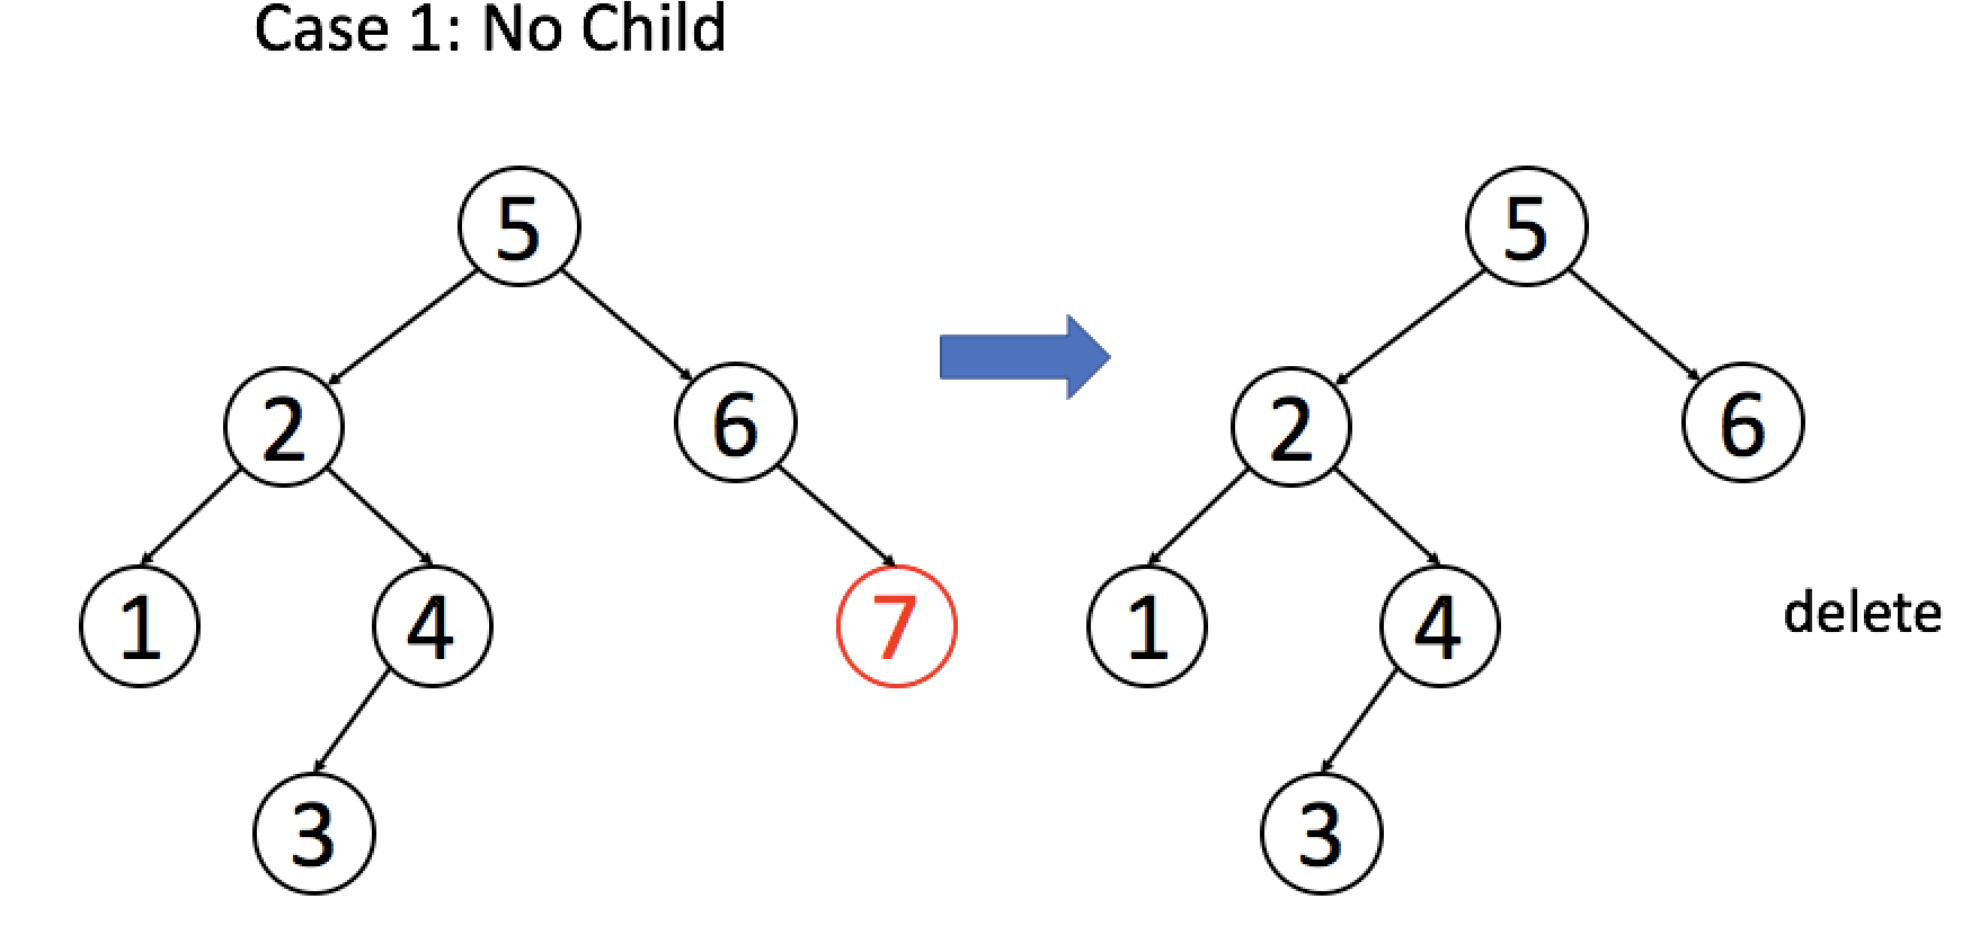
\includegraphics[width=.6\textwidth]{fig/BST_Delete_1.png}
\end{figure}
\begin{lstlisting}
if (root.left == null && root.right == null)
    return null;
\end{lstlisting}

情况 2:A 只有一个非空子节点,那么它要让这个孩子接替自己的位置。
\begin{figure}[H]
    \centering
    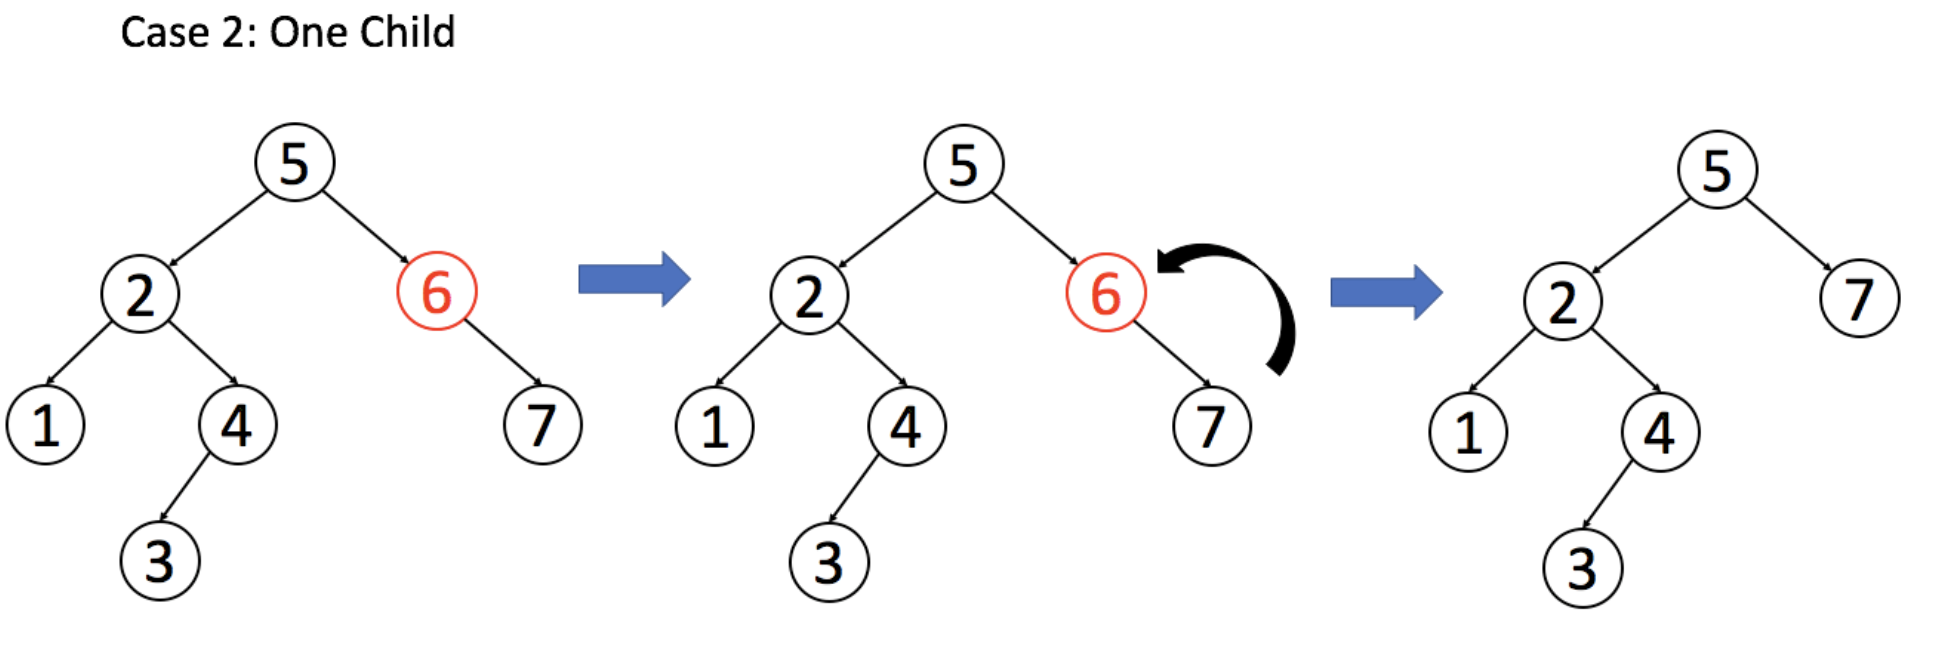
\includegraphics[width=.8\textwidth]{fig/BST_Delete_2.png}
\end{figure}
\begin{lstlisting}
// 排除了情况 1 之后
if (root.left == null) return root.right;
if (root.right == null) return root.left;
\end{lstlisting}

情况 3:A 有两个子节点,麻烦了,为了不破坏 BST 的性质,A 必须找到左子树中最大的那个节点,或者右子树中最小的那个节点来接替自己。我们以第二种方式讲解。
\begin{figure}[H]
    \centering
    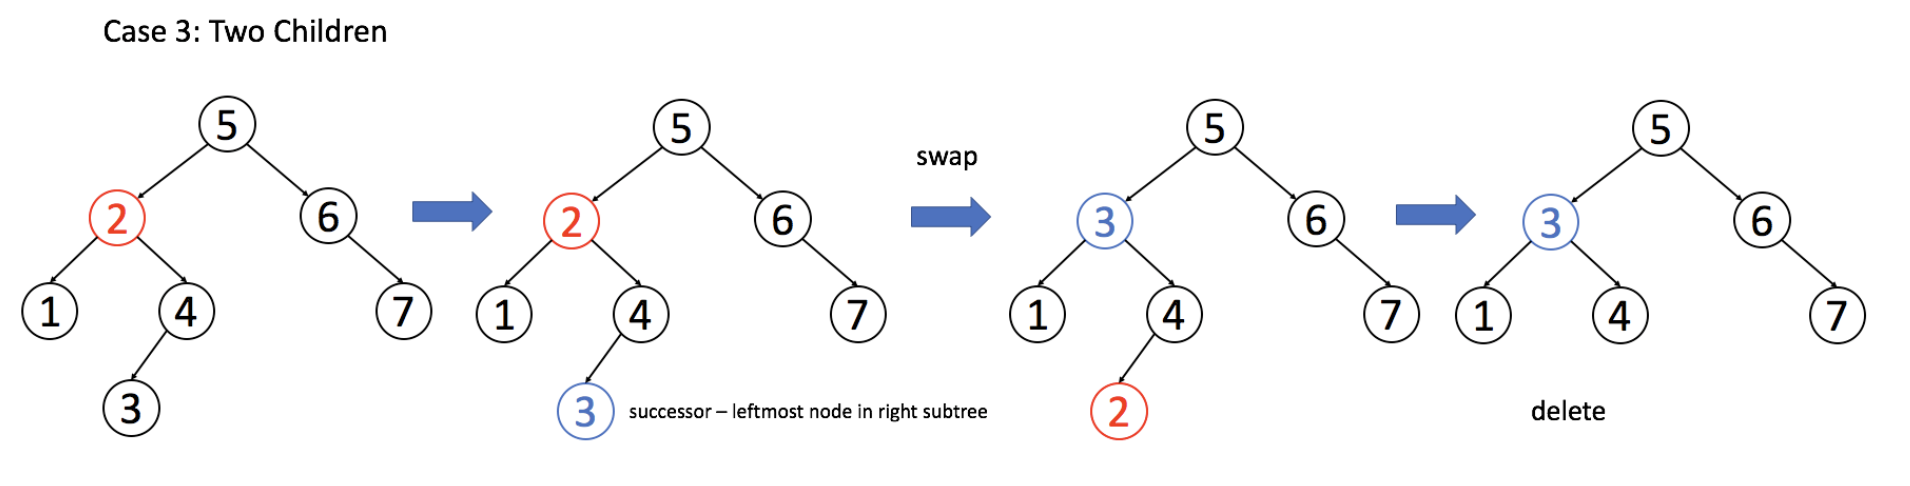
\includegraphics[width=1\textwidth]{fig/BST_Delete_3.png}
\end{figure}
\begin{lstlisting}
if (root.left != null && root.right != null) {
    // 找到右子树的最小节点
    TreeNode minNode = getMin(root.right);
    // 把 root 改成 minNode
    root.val = minNode.val;
    // 转而去删除 minNode
    root.right = deleteNode(root.right, minNode.val);
}
\end{lstlisting}

三种情况分析完毕,填入框架,简化一下代码:
\begin{lstlisting}
TreeNode deleteNode(TreeNode root, int key) {
    if (root == null) return null;
    if (root.val == key) {
        // 这两个 if 把情况 1 和 2 都正确处理了
        if (root.left == null) return root.right;
        if (root.right == null) return root.left;
        // 处理情况 3
        TreeNode minNode = getMin(root.right);
        root.val = minNode.val;
        root.right = deleteNode(root.right, minNode.val);
    } else if (root.val > key) {
        root.left = deleteNode(root.left, key);
    } else if (root.val < key) {
        root.right = deleteNode(root.right, key);
    }
    return root;
}

TreeNode getMin(TreeNode node) {
    // BST 最左边的就是最小的
    while (node.left != null) node = node.left;
    return node;
} 
\end{lstlisting}
删除操作就完成了。注意一下,这个删除操作并不完美,因为我们一般不会通过 root.val = minNode.val 修改节点内部的值来交换节点,而是通过一系列略微复杂的链表操作交换 root 和 minNode 两个节点。因为具体应用中,val 域可能会很大,修改起来很耗时,而链表操作无非改一改指针,而不会去碰内部数据。

但这里忽略这个细节,旨在突出 BST 基本操作的共性,以及借助框架逐层细化问题的思维方式。

\subsubsection{BST 总结}
通过这篇文章,你学会了如下几个技巧:
\begin{itemize}
\setlength{\itemsep}{0pt}
\setlength{\parsep}{0pt}
\setlength{\parskip}{0pt}
    \item 二叉树算法设计的总路线:把当前节点要做的事做好,其他的交给递归框架,不用当前节点操心。
    \item 如果当前节点会对下面的子节点有整体影响,可以通过辅助函数增长参数列表,借助参数传递信息。
    \item 在二叉树框架之上,扩展出一套 BST 遍历框架:
    \begin{lstlisting}
void BST(TreeNode root, int target) {
    if (root.val == target)
        // 找到目标,做点什么
    if (root.val < target) 
        BST(root.right, target);
    if (root.val > target)
        BST(root.left, target);
}
\end{lstlisting}
    \item 掌握了 BST 的基本操作。
\end{itemize}

\section{单调栈}
\url{https://github.com/labuladong/fucking-algorithm/blob/master/%E6%95%B0%E6%8D%AE%E7%BB%93%E6%9E%84%E7%B3%BB%E5%88%97/%E5%8D%95%E8%B0%83%E6%A0%88.md}

代码见:\url{codes/monotonic_stack.py}

\subsection{单调栈的定义和应用场景}
栈(stack)是很简单的一种数据结构,先进后出的逻辑顺序,符合某些问题的特点,比如说函数调用栈。

单调栈实际上就是栈,只是利用了一些巧妙的逻辑,使得每次新元素入栈后,\textbf{栈内的元素都保持有序(单调递增或单调递减)}。

听起来有点像堆(heap)?不是的,单调栈用途不太广泛,只处理一种典型的问题,叫做 Next Greater Element。本文用讲解单调队列的算法模版解决这类问题,并且探讨处理「循环数组」的策略。

\subsection{Next Greater Number}
首先,讲解 Next Greater Number 的原始问题:给你一个数组,返回一个等长的数组,对应索引存储着下一个更大元素,如果没有更大的元素,就存 -1。不好用语言解释清楚,直接上一个例子:

例:给你一个数组 [2,1,2,4,3],你返回数组 [4,2,4,-1,-1]。

解释:第一个 2 后面比 2 大的数是 4; 1 后面比 1 大的数是 2;第二个 2 后面比 2 大的数是 4; 4 后面没有比 4 大的数,填 -1;3 后面没有比 3 大的数,填 -1。

这道题的暴力解法很好想到,就是对每个元素后面都进行扫描,找到第一个更大的元素就行了。但是暴力解法的时间复杂度是 $O(n^2)$。

这个问题可以这样抽象思考:把数组的元素想象成并列站立的人,元素大小想象成人的身高。这些人面对你站成一列,如何求元素「2」的 Next Greater Number 呢?很简单,如果能够看到元素「2」,那么他后面可见的第一个人就是「2」的 Next Greater Number,因为比「2」小的元素身高不够,都被「2」挡住了,第一个露出来的就是答案。

这个情景很好理解吧?带着这个抽象的情景,先来看下代码。
\begin{lstlisting}
vector<int> nextGreaterElement(vector<int>& nums) {
    vector<int> ans(nums.size()); // 存放答案的数组
    stack<int> s;
    for (int i = nums.size() - 1; i >= 0; i--) { // 倒着往栈里放
        while (!s.empty() && s.top() <= nums[i]) { // 判定个子高矮
            s.pop(); // 矮个起开,反正也被挡着了。。。
        }
        ans[i] = s.empty() ? -1 : s.top(); // 这个元素身后的第一个高个
        s.push(nums[i]); // 进队,接受之后的身高判定吧!
    }
    return ans;
}
\end{lstlisting}

这就是单调队列解决问题的模板。for 循环要从后往前扫描元素,因为我们借助的是栈的结构,倒着入栈,其实是正着出栈。while 循环是把两个“高个”元素之间的元素排除,因为他们的存在没有意义,前面挡着个“更高”的元素,所以他们不可能被作为后续进来的元素的 Next Great Number 了。

这个算法的时间复杂度不是那么直观,如果你看到 for 循环嵌套 while 循环,可能认为这个算法的复杂度也是 $O(n^2)$,但是实际上这个算法的复杂度只有 $O(n)$。

分析它的时间复杂度,要从整体来看:总共有 n 个元素,每个元素都被 push 入栈了一次,而最多会被 pop 一次,没有任何冗余操作。所以总的计算规模是和元素规模 n 成正比的,也就是 $O(n)$ 的复杂度。

现在,你已经掌握了单调栈的使用技巧,来一个简单的变形来加深一下理解。

\subsection{应用场景}
\subsubsection{更缓和的天气}
给你一个数组 T = [73, 74, 75, 71, 69, 72, 76, 73],这个数组存放的是近几天的天气气温(这气温是铁板烧?不是的,这里用的华氏度)。你返回一个数组,计算:对于每一天,你还要至少等多少天才能等到一个更暖和的气温;如果等不到那一天,填 0 。

举例:给你 T = [73, 74, 75, 71, 69, 72, 76, 73],你返回 [1, 1, 4, 2, 1, 1, 0, 0]。

解释:第一天 73 华氏度,第二天 74 华氏度,比 73 大,所以对于第一天,只要等一天就能等到一个更暖和的气温。后面的同理。

你已经对 Next Greater Number 类型问题有些敏感了,这个问题本质上也是找 Next Greater Number,只不过现在不是问你 Next Greater Number 是多少,而是问你当前距离 Next Greater Number 的距离而已。

相同类型的问题,相同的思路,直接调用单调栈的算法模板,稍作改动就可以啦,直接上代码把。
\begin{lstlisting}
vector<int> dailyTemperatures(vector<int>& T) {
    vector<int> ans(T.size());
    stack<int> s; // 这里放元素索引,而不是元素
    for (int i = T.size() - 1; i >= 0; i--) {
        while (!s.empty() && T[s.top()] <= T[i]) {
            s.pop();
        }
        ans[i] = s.empty() ? 0 : (s.top() - i); // 得到索引间距
        s.push(i); // 加入索引,而不是元素
    }
    return ans;
}
\end{lstlisting}

\subsubsection{处理循环数组}
同样是 Next Greater Number,现在假设给你的数组是个环形的,如何处理?

给你一个数组 [2,1,2,4,3],你返回数组 [4,2,4,-1,4]。拥有了环形属性,最后一个元素 3 绕了一圈后找到了比自己大的元素 4 。

首先,计算机的内存都是线性的,没有真正意义上的环形数组,但是我们可以模拟出环形数组的效果,一般是通过 \% 运算符求模(余数),获得环形特效:
\begin{lstlisting}
int[] arr = {1,2,3,4,5};
int n = arr.length, index = 0;
while (true) {
    print(arr[index % n]);
    index++;
}
\end{lstlisting}

回到 Next Greater Number 的问题,增加了环形属性后,问题的难点在于:这个 Next 的意义不仅仅是当前元素的右边了,有可能出现在当前元素的左边(如上例)。

明确问题,问题就已经解决了一半了。我们可以考虑这样的思路:\textbf{将原始数组“翻倍”,就是在后面再接一个原始数组},这样的话,按照之前“比身高”的流程,每个元素不仅可以比较自己右边的元素,而且也可以和左边的元素比较了。

怎么实现呢?你当然可以把这个双倍长度的数组构造出来,然后套用算法模板。但是,我们可以不用构造新数组,而是利用循环数组的技巧来模拟。直接看代码吧:
\begin{lstlisting}
vector<int> nextGreaterElements(vector<int>& nums) {
    int n = nums.size();
    vector<int> res(n); // 存放结果
    stack<int> s;
    // 假装这个数组长度翻倍了
    for (int i = 2 * n - 1; i >= 0; i--) {
        while (!s.empty() && s.top() <= nums[i % n])
            s.pop();
        res[i % n] = s.empty() ? -1 : s.top();
        s.push(nums[i % n]);
    }
    return res;
}
\end{lstlisting}

\section{单调队列}
\url{https://github.com/labuladong/fucking-algorithm/blob/master/%E6%95%B0%E6%8D%AE%E7%BB%93%E6%9E%84%E7%B3%BB%E5%88%97/%E5%8D%95%E8%B0%83%E9%98%9F%E5%88%97.md}

\subsection{单调队列的定义和应用场景}
「单调队列」,只是使用了一点巧妙的方法,使得队列中的元素单调递增(或递减)。这个数据结构有什么用?可以解决滑动窗口的一系列问题。

看一道 LeetCode 题目,难度 hard:
\begin{figure}[H]
    \centering
    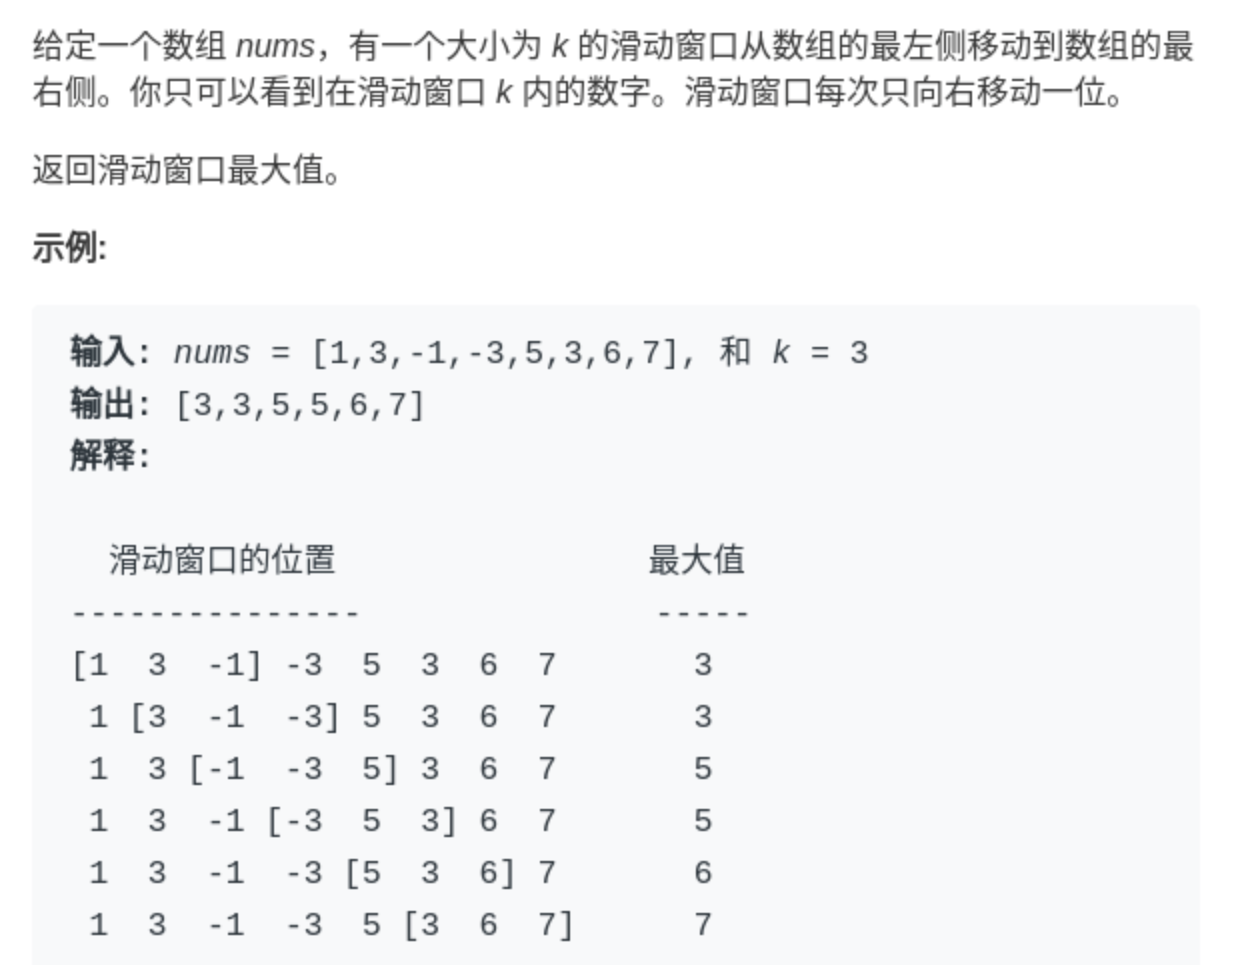
\includegraphics[width=.8\textwidth]{fig/monotonic_queue_1.png}
\end{figure}

\subsection{搭建解题框架}
这道题不复杂,难点在于如何在 O(1) 时间算出每个「窗口」中的最大值,使得整个算法在线性时间完成。在之前我们探讨过类似的场景,得到一个结论:

\textbf{在一堆数字中,已知最值,如果给这堆数添加一个数,那么比较一下就可以很快算出最值;但如果减少一个数,就不一定能很快得到最值了,而要遍历所有数重新找最值}。

回到这道题的场景,每个窗口前进的时候,要添加一个数同时减少一个数,所以想在 O(1) 的时间得出新的最值,就需要「单调队列」这种特殊的数据结构来辅助了。

一个普通的队列一定有这两个操作:
\begin{lstlisting}
class Queue {
    void push(int n);
    // 或 enqueue,在队尾加入元素 n
    void pop();
    // 或 dequeue,删除队头元素
}
\end{lstlisting}

一个「单调队列」的操作也差不多:
\begin{lstlisting}
class MonotonicQueue {
    // 在队尾添加元素 n
    void push(int n);
    // 返回当前队列中的最大值
    int max();
    // 队头元素如果是 n,删除它
    void pop(int n);
}
\end{lstlisting}

当然,这几个 API 的实现方法肯定跟一般的 Queue 不一样,不过我们暂且不管,而且认为这几个操作的时间复杂度都是 O(1),先把这道「滑动窗口」问题的解答框架搭出来:
\begin{lstlisting}
vector<int> maxSlidingWindow(vector<int>& nums, int k) {
    MonotonicQueue window;
    vector<int> res;
    for (int i = 0; i < nums.size(); i++) {
        if (i < k - 1) { //先把窗口的前 k - 1 填满
            window.push(nums[i]);
        } else { // 窗口开始向前滑动
            window.push(nums[i]);
            res.push_back(window.max());
            window.pop(nums[i - k + 1]);
            // nums[i - k + 1] 就是窗口最后的元素
        }
    }
    return res;
}
\end{lstlisting}
\begin{figure}[H]
    \centering
    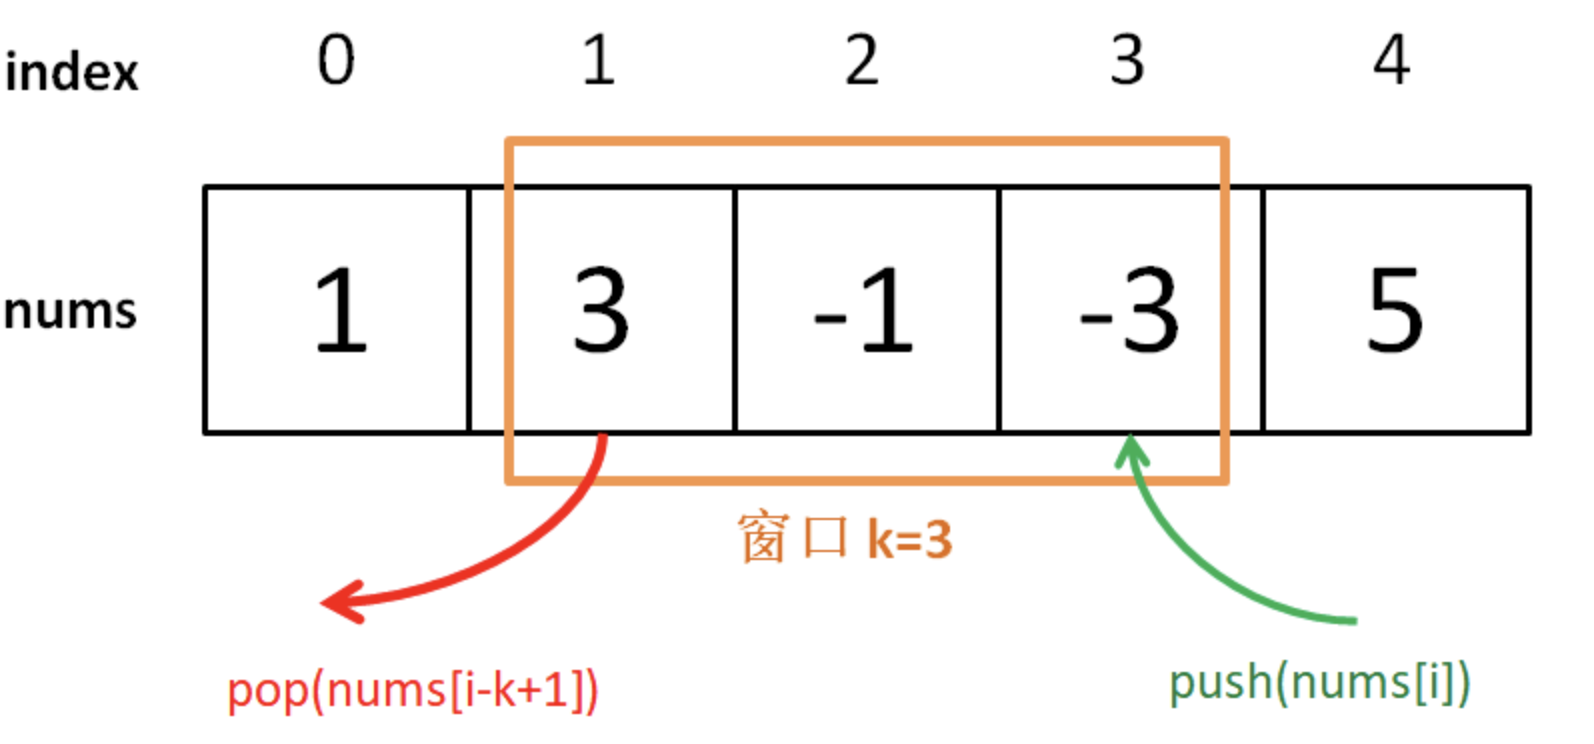
\includegraphics[width=.5\textwidth]{fig/monotonic_queue_2.png}
\end{figure}

\subsection{实现单调队列数据结构}
首先我们要认识另一种数据结构:deque,即双端队列。很简单:
\begin{lstlisting}
class deque {
    // 在队头插入元素 n
    void push_front(int n);
    // 在队尾插入元素 n
    void push_back(int n);
    // 在队头删除元素
    void pop_front();
    // 在队尾删除元素
    void pop_back();
    // 返回队头元素
    int front();
    // 返回队尾元素
    int back();
}
\end{lstlisting}
而且,这些操作的复杂度都是 O(1)。这其实不是啥稀奇的数据结构,用链表作为底层结构的话,很容易实现这些功能。

「单调队列」的核心思路和「单调栈」类似。单调队列的 push 方法依然在队尾添加元素,但是要把前面比新元素小的元素都删掉:
\begin{lstlisting}
class MonotonicQueue {
private:
    deque<int> data;
public:
    void push(int n) {
        while (!data.empty() && data.back() < n) 
            data.pop_back();
        data.push_back(n);
    }
};
\end{lstlisting}
你可以想象,加入数字的大小代表人的体重,把前面体重不足的都压扁了,直到遇到更大的量级才停住。

如果每个元素被加入时都这样操作,最终单调队列中的元素大小就会保持一个单调递减的顺序,因此我们的 max() API 可以可以这样写:
\begin{lstlisting}
int max() {
    return data.front();
}
\end{lstlisting}

pop() API 在队头删除元素 n,也很好写:
\begin{lstlisting}
int max() {
    return data.front();
}
\end{lstlisting}

pop() API 在队头删除元素 n,也很好写:
\begin{lstlisting}
void pop(int n) {
    if (!data.empty() && data.front() == n)
        data.pop_front();
}
\end{lstlisting}

之所以要判断 data.front() == n,是因为我们想删除的队头元素 n 可能已经被「压扁」了,这时候就不用删除了:

至此,单调队列设计完毕,看下完整的解题代码:
\begin{lstlisting}
class MonotonicQueue {
private:
    deque<int> data;
public:
    void push(int n) {
        while (!data.empty() && data.back() < n) 
            data.pop_back();
        data.push_back(n);
    }
    
    int max() { return data.front(); }
    
    void pop(int n) {
        if (!data.empty() && data.front() == n)
            data.pop_front();
    }
};

vector<int> maxSlidingWindow(vector<int>& nums, int k) {
    MonotonicQueue window;
    vector<int> res;
    for (int i = 0; i < nums.size(); i++) {
        if (i < k - 1) { //先填满窗口的前 k - 1
            window.push(nums[i]);
        } else { // 窗口向前滑动
            window.push(nums[i]);
            res.push_back(window.max());
            window.pop(nums[i - k + 1]);
        }
    }
    return res;
}
\end{lstlisting}

\subsection{算法复杂度分析}
读者可能疑惑,push 操作中含有 while 循环,时间复杂度不是 O(1) 呀,那么本算法的时间复杂度应该不是线性时间吧?

单独看 push 操作的复杂度确实不是 O(1),但是算法整体的复杂度依然是 O(N) 线性时间。要这样想,nums 中的每个元素最多被 push\_back 和 pop\_back 一次,没有任何多余操作,所以整体的复杂度还是 O(N)。

空间复杂度就很简单了,就是窗口的大小 O(k)。

\subsection{总结}
有的读者可能觉得「单调队列」和「优先级队列」比较像,实际上差别很大的。

单调队列在添加元素的时候靠删除元素保持队列的单调性,相当于抽取出某个函数中单调递增(或递减)的部分;而优先级队列(二叉堆)相当于自动排序,差别大了去了。

\section{设计Twitter}
\subsection{题目及应用场景简介}
Twitter 和微博功能差不多,我们主要要实现这样几个 API:
\begin{lstlisting}
class Twitter {
    /** user 发表一条 tweet 动态 */
    public void postTweet(int userId, int tweetId) {}
    
    /** 返回该 user 关注的人(包括他自己)最近的动态 id,
    最多 10 条,而且这些动态必须按从新到旧的时间线顺序排列。*/
    public List<Integer> getNewsFeed(int userId) {}
    
    /** follower 关注 followee,如果 Id 不存在则新建 */
    public void follow(int followerId, int followeeId) {}
    
    /** follower 取关 followee,如果 Id 不存在则什么都不做 */
    public void unfollow(int followerId, int followeeId) {}
}
\end{lstlisting}

举个具体的例子,方便大家理解 API 的具体用法:
\begin{lstlisting}
Twitter twitter = new Twitter();

twitter.postTweet(1, 5);
// 用户 1 发送了一条新推文 5

twitter.getNewsFeed(1);
// return [5],因为自己是关注自己的

twitter.follow(1, 2);
// 用户 1 关注了用户 2

twitter.postTweet(2, 6);
// 用户2发送了一个新推文 (id = 6)

twitter.getNewsFeed(1);
// return [6, 5]
// 解释:用户 1 关注了自己和用户 2,所以返回他们的最近推文
// 而且 6 必须在 5 之前,因为 6 是最近发送的

twitter.unfollow(1, 2);
// 用户 1 取消关注了用户 2

twitter.getNewsFeed(1);
// return [5]
\end{lstlisting}
这个场景在我们的现实生活中非常常见。拿朋友圈举例,比如我刚加到女神的微信,然后我去刷新一下我的朋友圈动态,那么女神的动态就会出现在我的动态列表,而且会和其他动态按时间排好序。只不过 Twitter 是单向关注,微信好友相当于双向关注。除非,被屏蔽...

这几个 API 中大部分都很好实现,最核心的功能难点应该是 getNewsFeed,因为返回的结果必须在时间上有序,但问题是用户的关注是动态变化的,怎么办?

这里就涉及到算法了:\textbf{如果我们把每个用户各自的推文存储在链表里,每个链表节点存储文章 id 和一个时间戳 time(记录发帖时间以便比较),而且这个链表是按 time 有序的},那么如果某个用户关注了 k 个用户,我们就可以用\textbf{合并 k 个有序链表}的算法合并出有序的推文列表,正确地 getNewsFeed 了!

具体的算法等会讲解。不过,就算我们掌握了算法,应该如何编程表示用户 user 和推文动态 tweet 才能把算法流畅地用出来呢?这就涉及简单的面向对象设计了,下面我们来由浅入深,一步一步进行设计。

\subsection{面向对象设计}
根据刚才的分析,我们需要一个 User 类,储存 user 信息,还需要一个 Tweet 类,储存推文信息,并且要作为链表的节点。所以我们先搭建一下整体的框架:
\begin{lstlisting}
class Twitter {
    private static int timestamp = 0;
    private static class Tweet {}
    private static class User {}

    /* 还有那几个 API 方法 */
    public void postTweet(int userId, int tweetId) {}
    public List<Integer> getNewsFeed(int userId) {}
    public void follow(int followerId, int followeeId) {}
    public void unfollow(int followerId, int followeeId) {}
}
\end{lstlisting}
之所以要把 Tweet 和 User 类放到 Twitter 类里面,是因为 Tweet 类必须要用到一个全局时间戳 timestamp,而 User 类又需要用到 Tweet 类记录用户发送的推文,所以它们都作为内部类。不过为了清晰和简洁,下文会把每个内部类和 API 方法单独拿出来实现。

\subsubsection{Tweet 类的实现}
根据前面的分析,Tweet 类很容易实现:每个 Tweet 实例需要记录自己的 tweetId 和发表时间 time,而且作为链表节点,要有一个指向下一个节点的 next 指针。
\begin{lstlisting}
class Tweet {
    private int id;
    private int time;
    private Tweet next;

    // 需要传入推文内容(id)和发文时间
    public Tweet(int id, int time) {
        this.id = id;
        this.time = time;
        this.next = null;
    }
}
\end{lstlisting}

\subsubsection{User 类的实现}
我们根据实际场景想一想,一个用户需要存储的信息有 userId,关注列表,以及该用户发过的推文列表。其中关注列表应该用集合(Hash Set)这种数据结构来存,因为不能重复,而且需要快速查找;推文列表应该由链表这种数据结构储存,以便于进行有序合并的操作。画个图理解一下:
\begin{figure}[H]
    \centering
    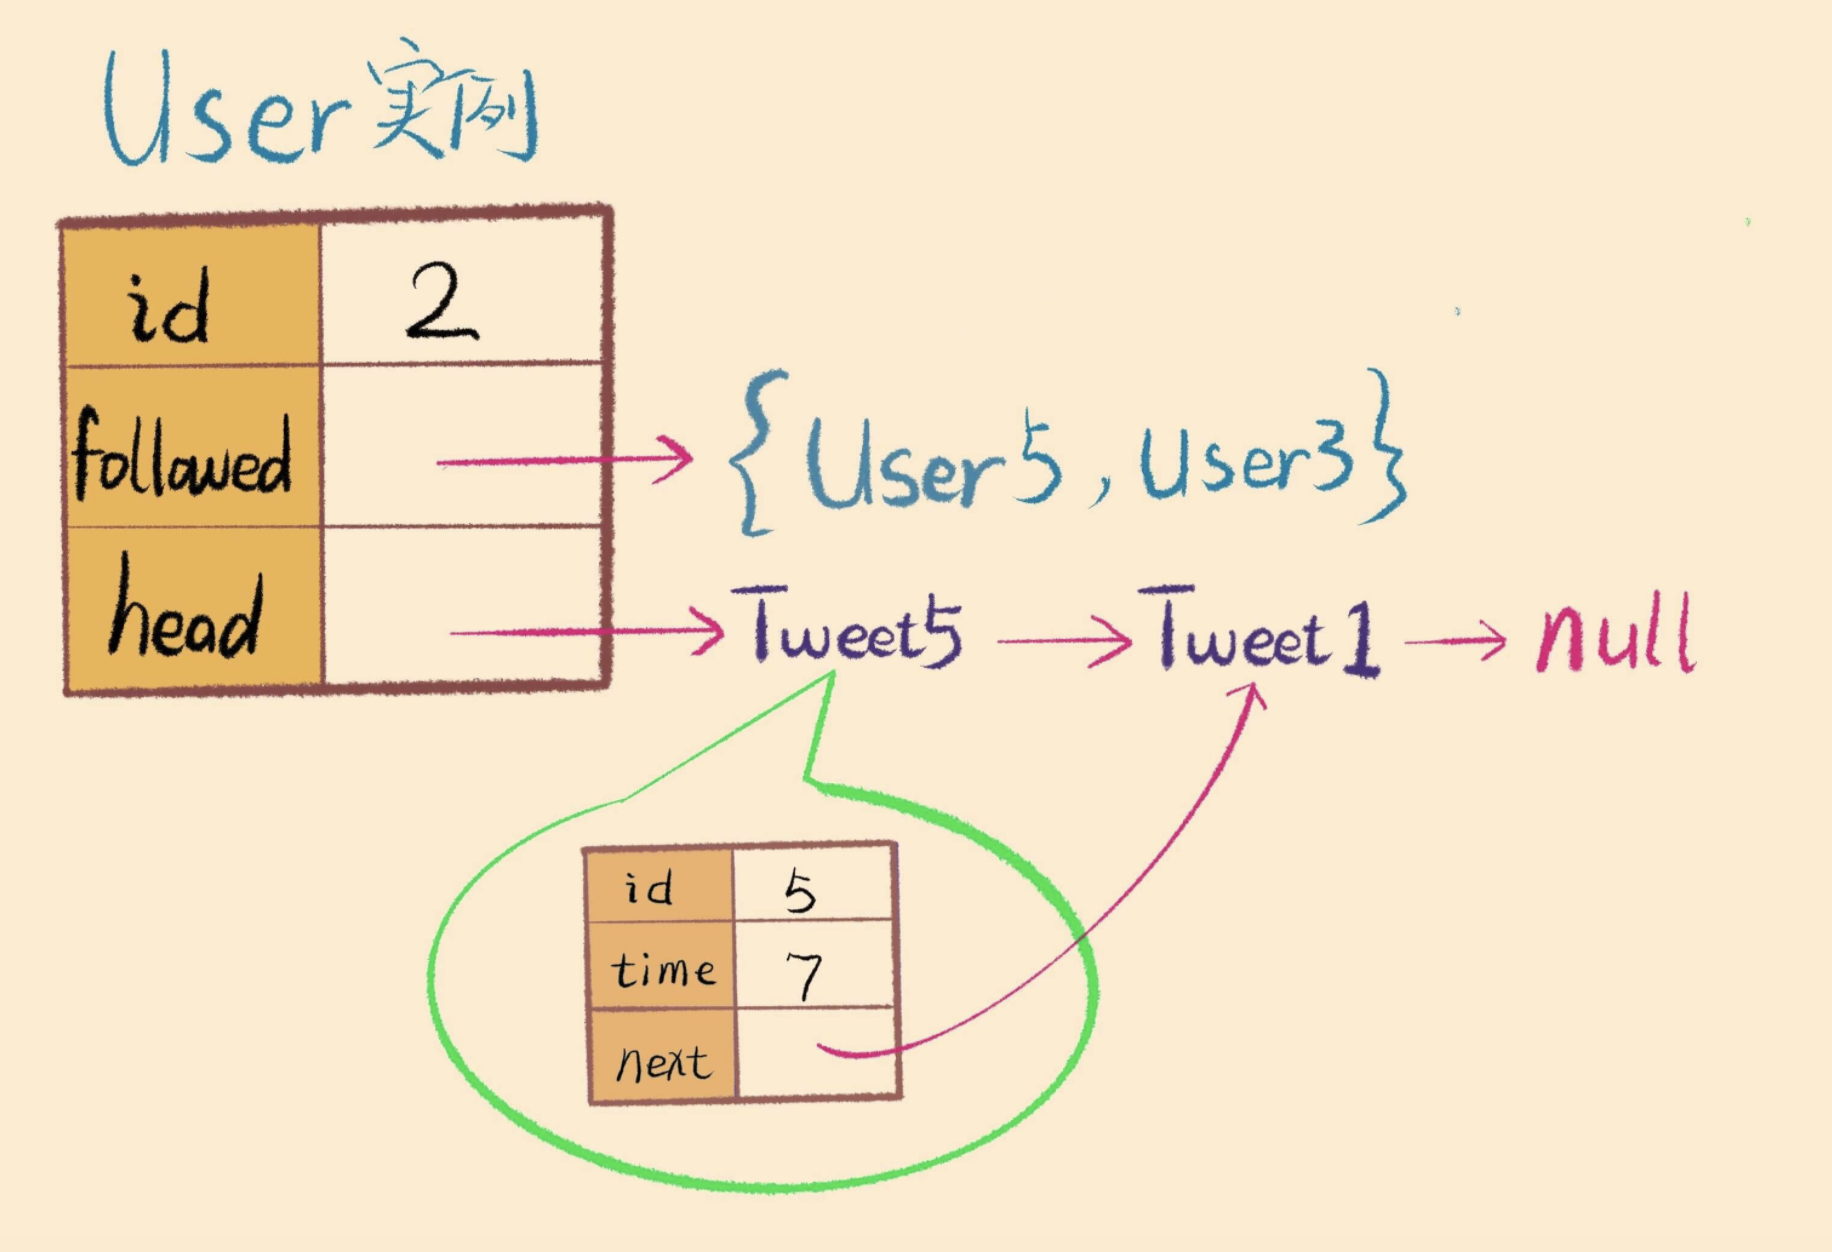
\includegraphics[width=.5\textwidth]{fig/Twitter_Design_1.png}
\end{figure}

除此之外,根据面向对象的设计原则,「关注」「取关」和「发文」应该是 User 的行为,况且关注列表和推文列表也存储在 User 类中,所以我们也应该给 User 添加 follow,unfollow 和 post 这几个方法:
\begin{lstlisting}
// static int timestamp = 0
class User {
    private int id;
    public Set<Integer> followed;
    // 用户发表的推文链表头结点
    public Tweet head;

    public User(int userId) {
        followed = new HashSet<>();
        this.id = userId;
        this.head = null;
        // 关注一下自己
        follow(id);
    }

    public void follow(int userId) {
        followed.add(userId);
    }

    public void unfollow(int userId) {
        // 不可以取关自己
        if (userId != this.id)
            followed.remove(userId);
    }

    public void post(int tweetId) {
        Tweet twt = new Tweet(tweetId, timestamp);
        timestamp++;
        // 将新建的推文插入链表头
        // 越靠前的推文 time 值越大
        twt.next = head;
        head = twt;
    }
}
\end{lstlisting}

\subsubsection{几个 API 方法的实现}
\begin{lstlisting}
class Twitter {
    private static int timestamp = 0;
    private static class Tweet {...}
    private static class User {...}

    // 我们需要一个映射将 userId 和 User 对象对应起来
    private HashMap<Integer, User> userMap = new HashMap<>();

    /** user 发表一条 tweet 动态 */
    public void postTweet(int userId, int tweetId) {
        // 若 userId 不存在,则新建
        if (!userMap.containsKey(userId))
            userMap.put(userId, new User(userId));
        User u = userMap.get(userId);
        u.post(tweetId);
    }
    
    /** follower 关注 followee */
    public void follow(int followerId, int followeeId) {
        // 若 follower 不存在,则新建
		if(!userMap.containsKey(followerId)){
			User u = new User(followerId);
			userMap.put(followerId, u);
		}
        // 若 followee 不存在,则新建
		if(!userMap.containsKey(followeeId)){
			User u = new User(followeeId);
			userMap.put(followeeId, u);
		}
		userMap.get(followerId).follow(followeeId);
    }
    
    /** follower 取关 followee,如果 Id 不存在则什么都不做 */
    public void unfollow(int followerId, int followeeId) {
        if (userMap.containsKey(followerId)) {
            User flwer = userMap.get(followerId);
            flwer.unfollow(followeeId);
        }
    }

    /** 返回该 user 关注的人(包括他自己)最近的动态 id,
    最多 10 条,而且这些动态必须按从新到旧的时间线顺序排列。*/
    public List<Integer> getNewsFeed(int userId) {
        // 需要理解算法,见下文
    }
}
\end{lstlisting}

\subsubsection{合并 k 个有序链表的算法设计}
实现\textbf{合并 k 个有序链表的算法需要用到优先级队列(Priority Queue)},这种数据结构是「二叉堆」最重要的应用,你可以理解为它可以对插入的元素自动排序。乱序的元素插入其中就被放到了正确的位置,可以按照从小到大(或从大到小)有序地取出元素。
\begin{lstlisting}
PriorityQueue pq
# 乱序插入
for i in {2,4,1,9,6}:
    pq.add(i)
while pq not empty:
    # 每次取出第一个(最小)元素
    print(pq.pop())

# 输出有序:1,2,4,6,9
\end{lstlisting}

借助这种牛逼的数据结构支持,我们就很容易实现这个核心功能了。注意我们把优先级队列设为按 time 属性从大到小降序排列,因为 time 越大意味着时间越近,应该排在前面:
\begin{lstlisting}
public List<Integer> getNewsFeed(int userId) {
    List<Integer> res = new ArrayList<>();
    if (!userMap.containsKey(userId)) return res;
    // 关注列表的用户 Id
    Set<Integer> users = userMap.get(userId).followed;
    // 自动通过 time 属性从大到小排序,容量为 users 的大小
    PriorityQueue<Tweet> pq = 
        new PriorityQueue<>(users.size(), (a, b)->(b.time - a.time));

    // 先将所有链表头节点插入优先级队列
    for (int id : users) {
        Tweet twt = userMap.get(id).head;
        if (twt == null) continue;
        pq.add(twt);
    }

    while (!pq.isEmpty()) {
        // 最多返回 10 条就够了
        if (res.size() == 10) break;
        // 弹出 time 值最大的(最近发表的)
        Tweet twt = pq.poll();
        res.add(twt.id);
        // 将下一篇 Tweet 插入进行排序
        if (twt.next != null) 
            pq.add(twt.next);
    }
    return res;
}
\end{lstlisting}

\begin{framed}
\textbf{理解:只需要将所有链表的头结点插入优先队列即可,并不需要将所有的链表的所有元素都插入优先队列。因为后续抽取最近的10条的时候,是将当前最新的 tweet 取出后,再插入该链表的 next 元素,这样就“自动”对 next 元素和队列中的其余元素进行了比较。
}
\end{framed}

\section{递归反转链表的一部分}
\url{https://github.com/labuladong/fucking-algorithm/blob/master/%E6%95%B0%E6%8D%AE%E7%BB%93%E6%9E%84%E7%B3%BB%E5%88%97/%E9%80%92%E5%BD%92%E5%8F%8D%E8%BD%AC%E9%93%BE%E8%A1%A8%E7%9A%84%E4%B8%80%E9%83%A8%E5%88%86.md}

反转单链表的迭代实现不是一个困难的事情,但是递归实现就有点难度了,如果再加一点难度,让你仅仅反转单链表中的一部分,你是否能够递归实现呢?

本文就来由浅入深,step by step 地解决这个问题。如果你还不会递归地反转单链表也没关系,本文会从递归反转整个单链表开始拓展,只要你明白单链表的结构,相信你能够有所收获。
\begin{lstlisting}
// 单链表节点的结构
public class ListNode {
    int val;
    ListNode next;
    ListNode(int x) { val = x; }
}
\end{lstlisting}

什么叫反转单链表的一部分呢,就是给你一个索引区间,让你把单链表中这部分元素反转,其他部分不变:
\begin{figure}[H]
    \centering
    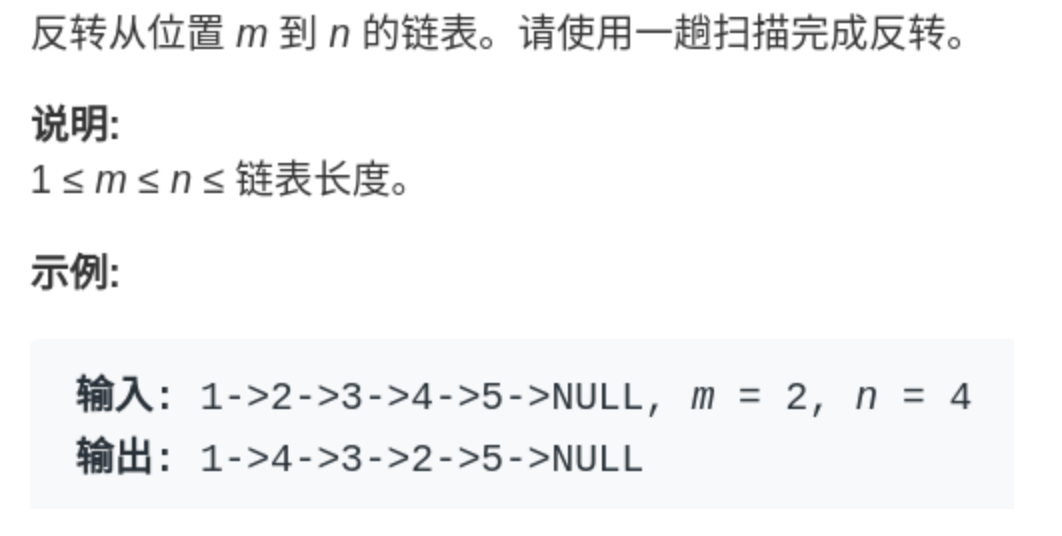
\includegraphics[width=.5\textwidth]{fig/Reverse_Single_List_1.png}
\end{figure}

注意这里的索引是从 1 开始的。迭代的思路大概是:先用一个 for 循环找到第 m 个位置,然后再用一个 for 循环将 m 和 n 之间的元素反转。但是我们的递归解法不用一个 for 循环,纯递归实现反转。

迭代实现思路看起来虽然简单,但是细节问题很多的,反而不容易写对。相反,递归实现就很简洁优美,下面就由浅入深,先从反转整个单链表说起。

\subsection{递归反转整个链表}
这个算法可能很多读者都听说过,这里详细介绍一下,先直接看实现代码:
\begin{lstlisting}
ListNode reverse(ListNode head) {
    if (head.next == null) return head;
    ListNode last = reverse(head.next);
    head.next.next = head;
    head.next = null;
    return last;
}
\end{lstlisting}
看起来是不是感觉不知所云,完全不能理解这样为什么能够反转链表?这就对了,这个算法常常拿来显示递归的巧妙和优美,我们下面来详细解释一下这段代码。

\textbf{对于递归算法,最重要的就是明确递归函数的定义}。具体来说,我们的 reverse 函数定义是这样的:

\textbf{输入一个节点 head,将「以 head 为起点」的链表反转,并返回反转之后的头结点}。

明白了函数的定义,在来看这个问题。比如说我们想反转这个链表:
\begin{figure}[H]
    \centering
    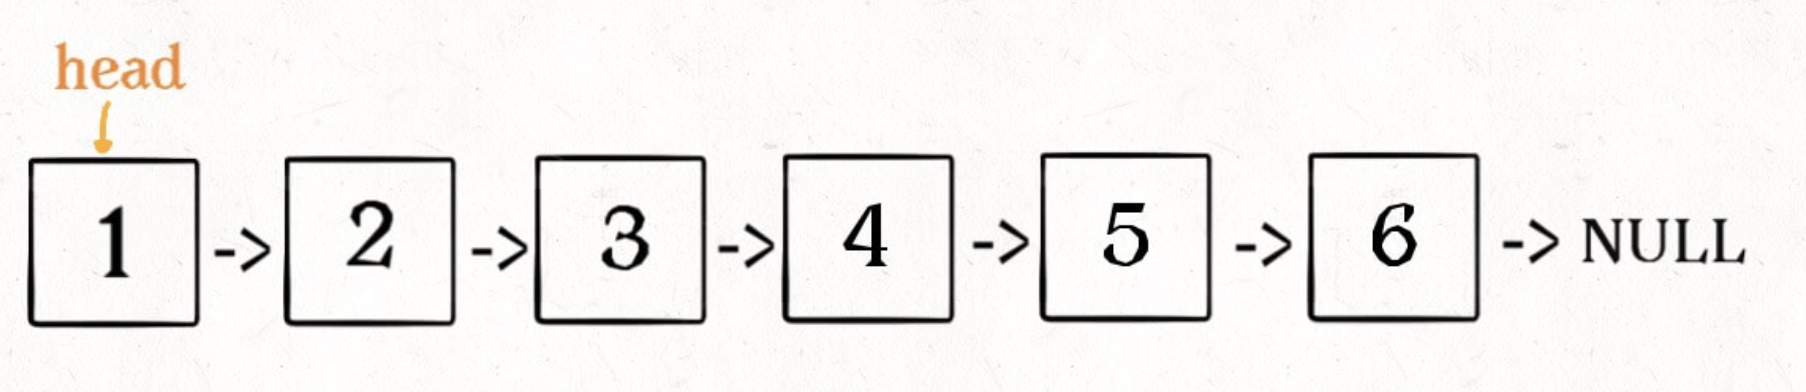
\includegraphics[width=.5\textwidth]{fig/Reverse_Single_List_2.png}
\end{figure}

那么输入 reverse(head) 后,会在这里进行递归:
\begin{lstlisting}
ListNode last = reverse(head.next);
\end{lstlisting}

不要跳进递归(你的脑袋能压几个栈呀?),而是要根据刚才的函数定义,来弄清楚这段代码会产生什么结果:
\begin{figure}[H]
    \centering
    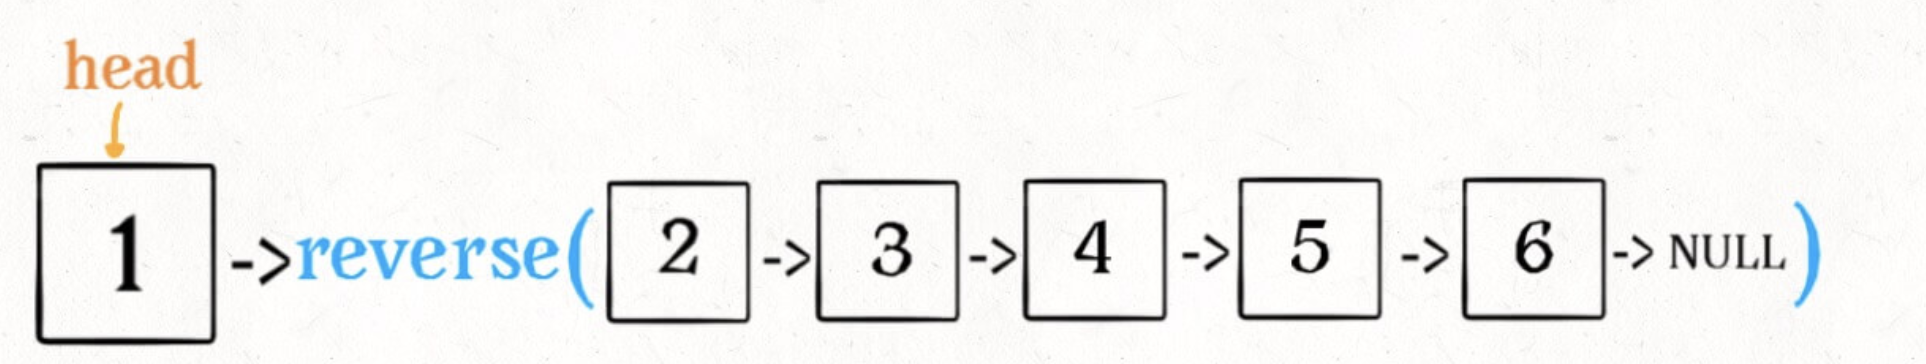
\includegraphics[width=.5\textwidth]{fig/Reverse_Single_List_3.png}
\end{figure}

这个 reverse(head.next) 执行完成后,整个链表就成了这样:
\begin{figure}[H]
    \centering
    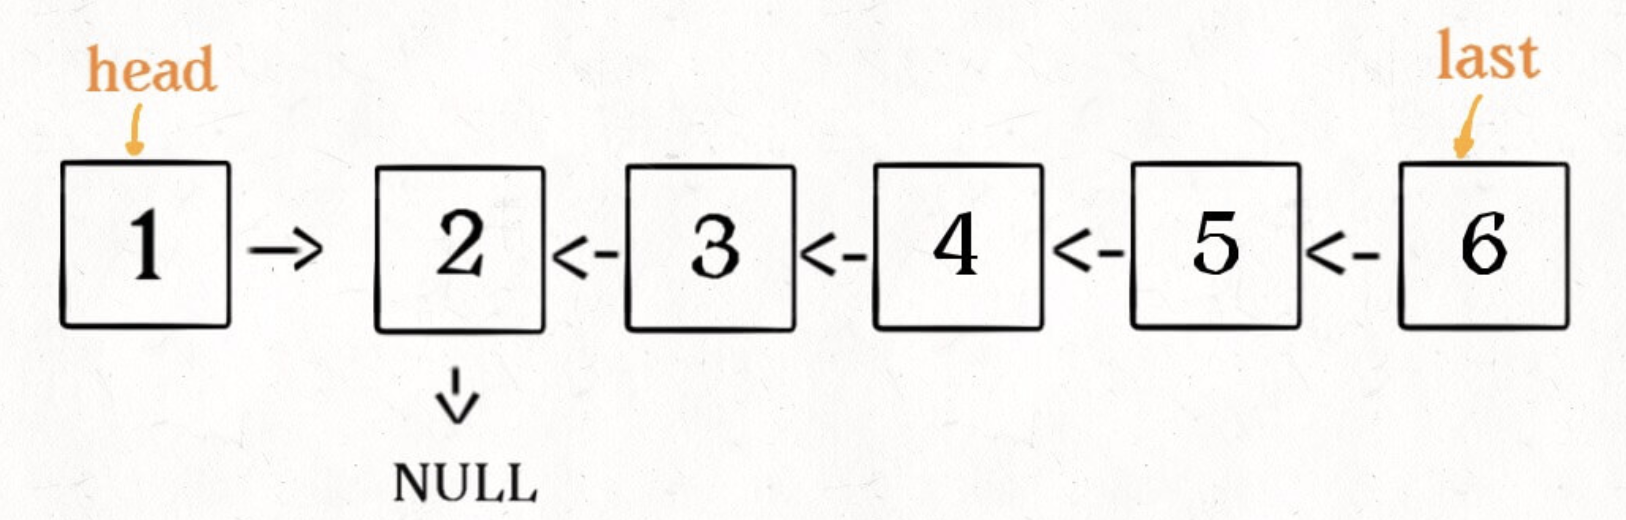
\includegraphics[width=.5\textwidth]{fig/Reverse_Single_List_4.png}
\end{figure}

并且根据函数定义,reverse 函数会返回反转之后的头结点,我们用变量 last 接收了。

现在再来看下面的代码:
\begin{lstlisting}
head.next.next = head;
\end{lstlisting}

\begin{figure}[H]
    \centering
    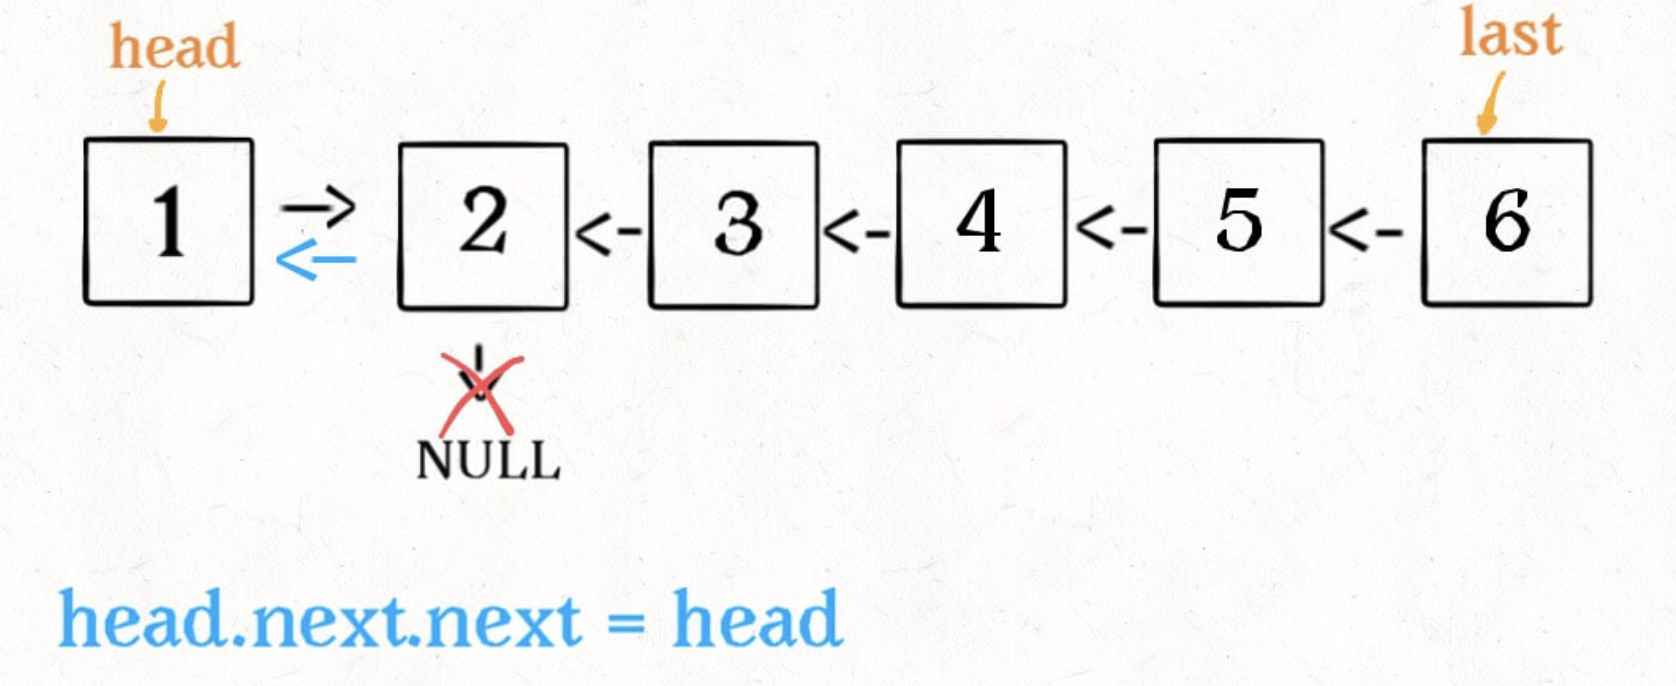
\includegraphics[width=.5\textwidth]{fig/Reverse_Single_List_5.png}
\end{figure}

接下来:
\begin{lstlisting}
head.next = null;
return last;
\end{lstlisting}

\begin{figure}[H]
    \centering
    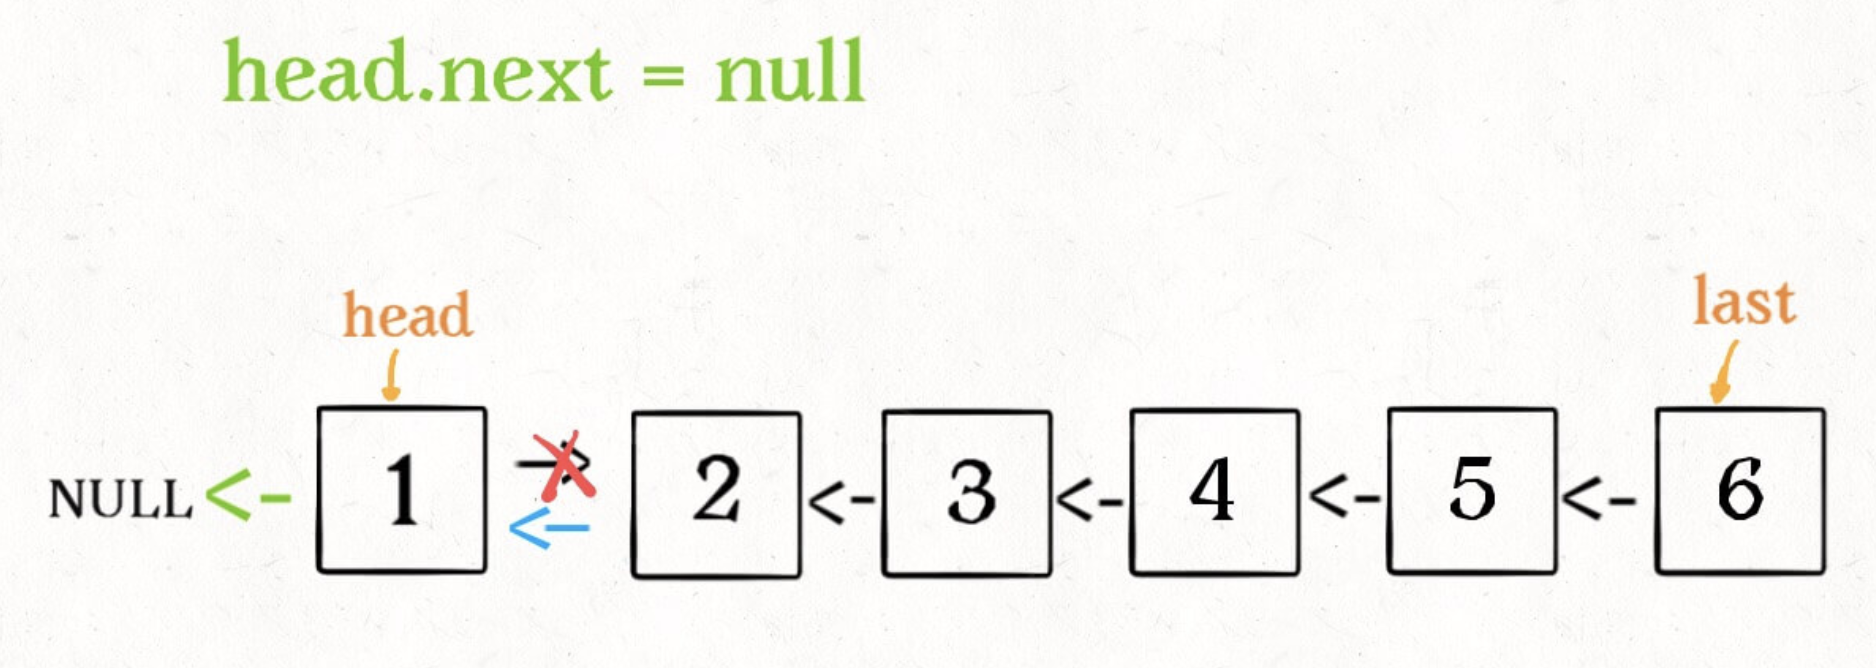
\includegraphics[width=.5\textwidth]{fig/Reverse_Single_List_6.png}
\end{figure}

神不神奇,这样整个链表就反转过来了!递归代码就是这么简洁优雅,不过其中有两个地方需要注意:

1、递归函数要有 base case,也就是这句:
\begin{lstlisting}
if (head.next == null) return head;
\end{lstlisting}
意思是如果链表只有一个节点的时候反转也是它自己,直接返回即可。

2、当链表递归反转之后,新的头结点是 last,而之前的 head 变成了最后一个节点,别忘了链表的末尾要指向 null:
\begin{lstlisting}
head.next = null;
\end{lstlisting}

\begin{framed}
\text{注意}:经过上述操作后,原链表的 head/tail 指针已经被破坏的,需要重置,见 \url{codes/reverse_list.py}
\begin{figure}[H]
    \centering
    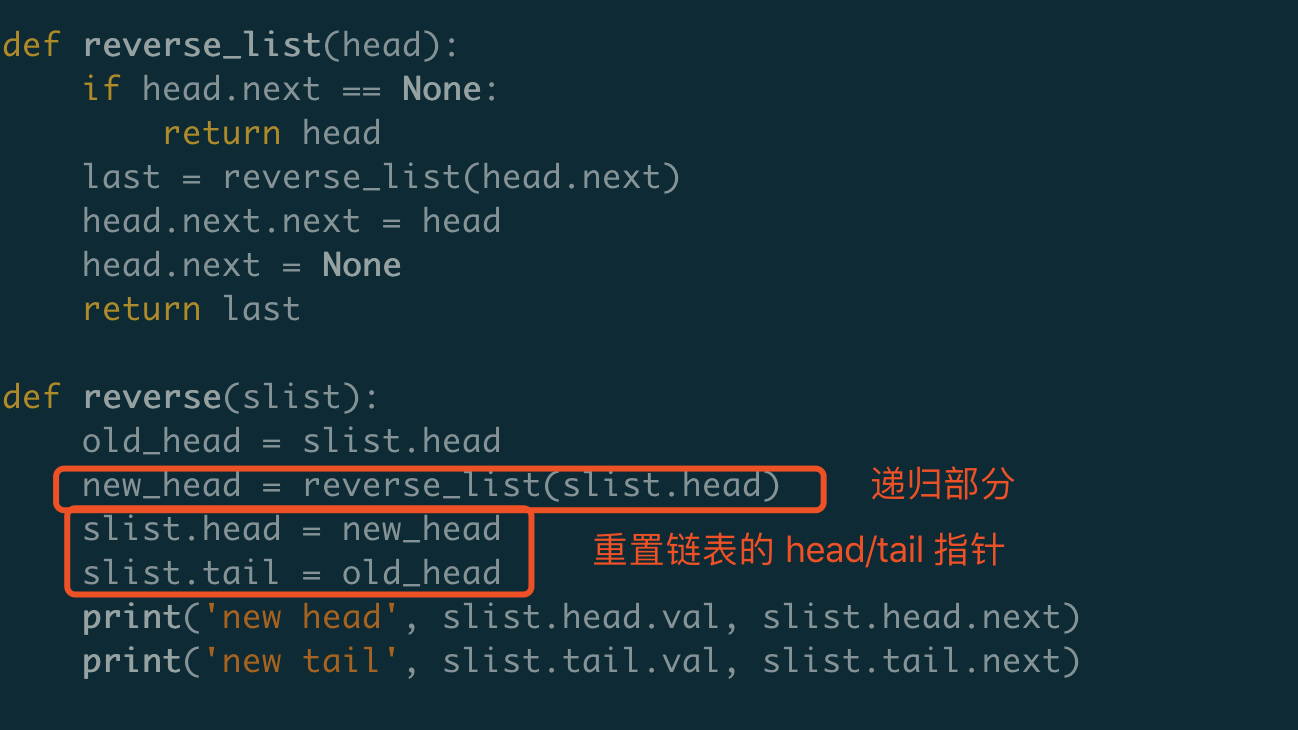
\includegraphics[width=.8\textwidth]{fig/Reverse_Single_List_9.png}
\end{figure}
\end{framed}

理解了这两点后,我们就可以进一步深入了,接下来的问题其实都是在这个算法上的扩展。

\subsection{反转链表前 N 个节点}
这次我们实现一个这样的函数:
\begin{lstlisting}
// 将链表的前 n 个节点反转(n <= 链表长度)
ListNode reverseN(ListNode head, int n)
\end{lstlisting}

比如说对于下图链表,执行 reverseN(head, 3):
\begin{figure}[H]
    \centering
    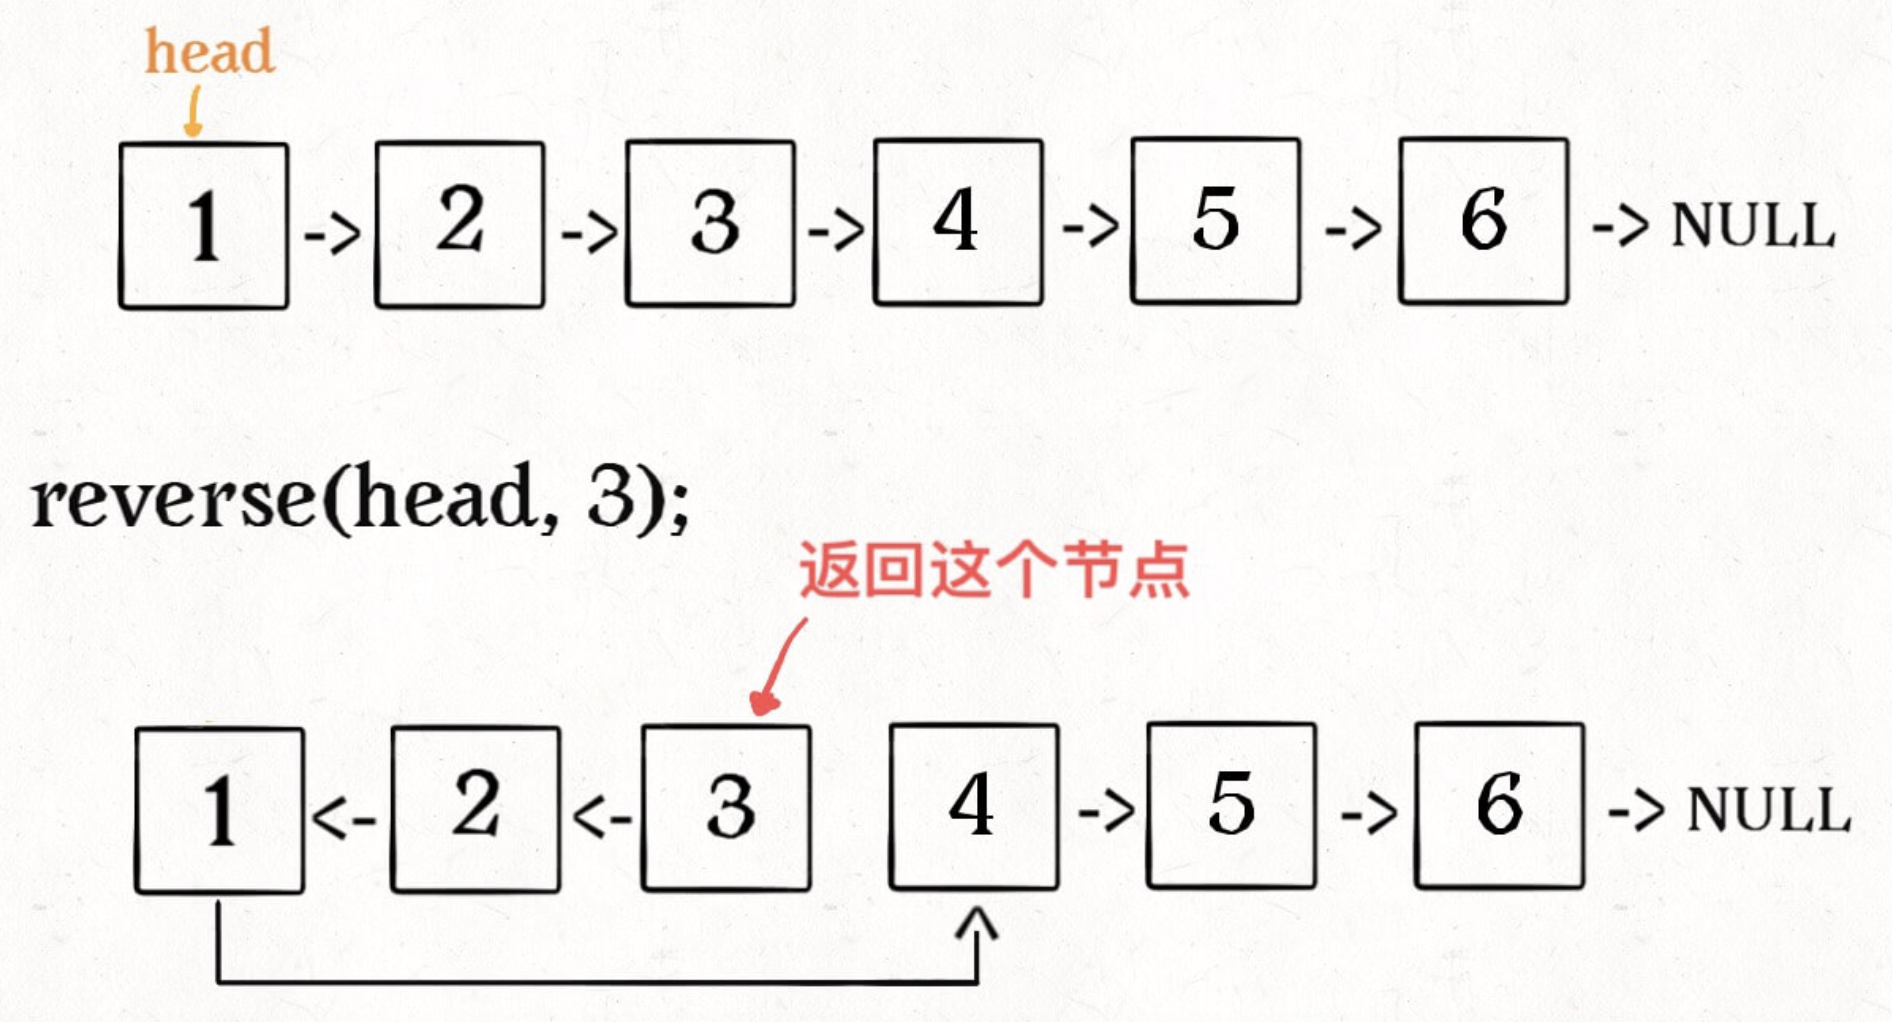
\includegraphics[width=.5\textwidth]{fig/Reverse_Single_List_7.png}
\end{figure}

解决思路和反转整个链表差不多,只要稍加修改即可:
\begin{lstlisting}
ListNode successor = null; // 后驱节点

// 反转以 head 为起点的 n 个节点,返回新的头结点
ListNode reverseN(ListNode head, int n) {
    if (n == 1) { 
        // 记录第 n + 1 个节点
        successor = head.next;
        return head;
    }
    // 以 head.next 为起点,需要反转前 n - 1 个节点
    ListNode last = reverseN(head.next, n - 1);

    head.next.next = head;
    // 让反转之后的 head 节点和后面的节点连起来
    head.next = successor;
    return last;
}    
\end{lstlisting}

具体的区别:

1、base case 变为 n == 1,反转一个元素,就是它本身,同时要记录后驱节点。

2、刚才我们直接把 head.next 设置为 null,因为整个链表反转后原来的 head 变成了整个链表的最后一个节点。但现在 head 节点在递归反转之后不一定是最后一个节点了,所以要记录后驱 successor(第 n + 1 个节点),反转之后将 head 连接上。
\begin{figure}[H]
    \centering
    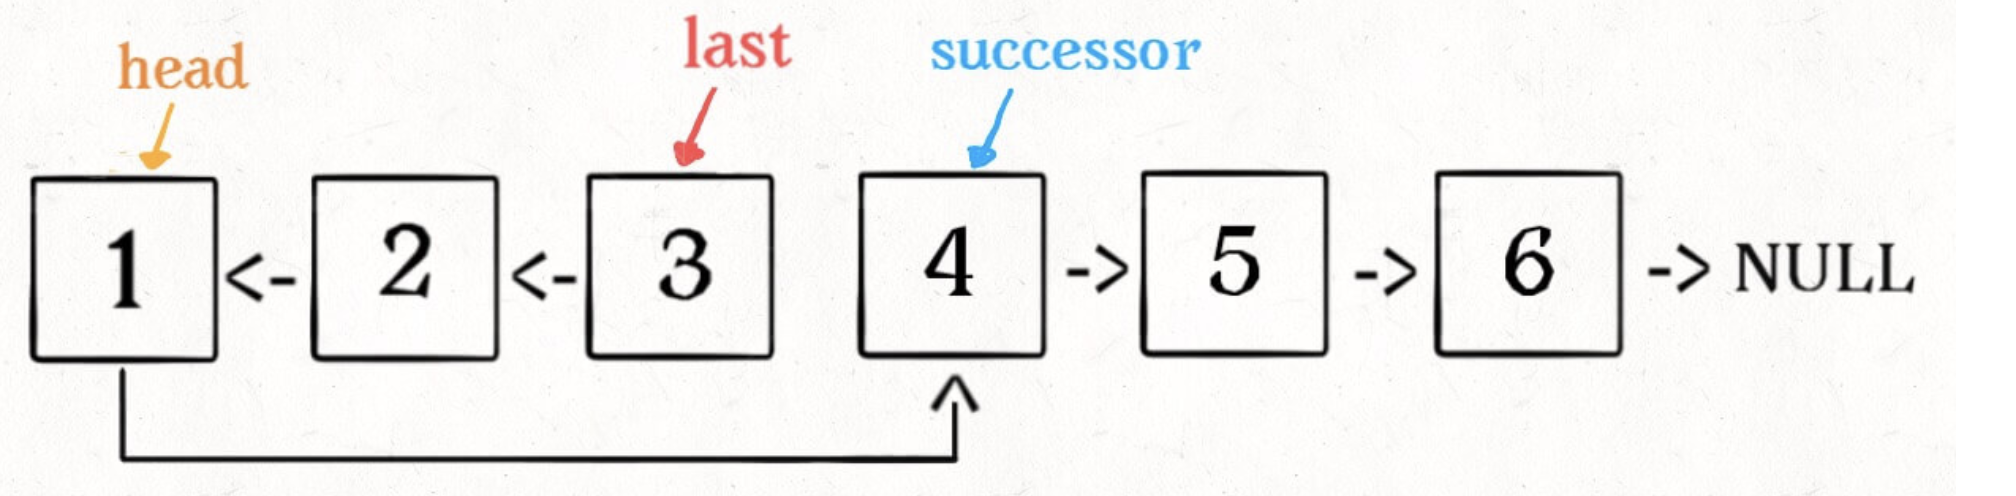
\includegraphics[width=.5\textwidth]{fig/Reverse_Single_List_8.png}
\end{figure}

\subsection{反转链表的一部分}
现在解决我们最开始提出的问题,给一个索引区间 [m,n](索引从 1 开始),仅仅反转区间中的链表元素。
\begin{lstlisting}
ListNode reverseBetween(ListNode head, int m, int n)
\end{lstlisting}

首先,如果 m == 1,就相当于反转链表开头的 n 个元素嘛,也就是我们刚才实现的功能:
\begin{lstlisting}
ListNode reverseBetween(ListNode head, int m, int n) {
    // base case
    if (m == 1) {
        // 相当于反转前 n 个元素
        return reverseN(head, n);
    }
    // ...
}
\end{lstlisting}

如果 m != 1 怎么办?如果我们把 head 的索引视为 1,那么我们是想从第 m 个元素开始反转对吧;如果把 head.next 的索引视为 1 呢?那么相对于 head.next,反转的区间应该是从第 m - 1 个元素开始的;那么对于 head.next.next 呢……

区别于迭代思想,这就是递归思想,所以我们可以完成代码:
\begin{lstlisting}
ListNode reverseBetween(ListNode head, int m, int n) {
    // base case
    if (m == 1) {
        return reverseN(head, n);
    }
    // 前进到反转的起点触发 base case
    head.next = reverseBetween(head.next, m - 1, n - 1);
    return head;
}
\end{lstlisting}

\subsection{总结}
递归的思想相对迭代思想,稍微有点难以理解,处理的技巧是:不要跳进递归,而是利用明确的定义来实现算法逻辑。

处理看起来比较困难的问题,可以尝试化整为零,把一些简单的解法进行修改,解决困难的问题。

值得一提的是,递归操作链表并不高效。和迭代解法相比,虽然时间复杂度都是 O(N),但是迭代解法的空间复杂度是 O(1),而递归解法需要堆栈,空间复杂度是 O(N)。所以递归操作链表可以作为对递归算法的练习或者拿去和小伙伴装逼,但是考虑效率的话还是使用迭代算法更好。

\section{队列实现栈和栈实现队列}
\url{https://github.com/labuladong/fucking-algorithm/blob/master/%E6%95%B0%E6%8D%AE%E7%BB%93%E6%9E%84%E7%B3%BB%E5%88%97/%E9%98%9F%E5%88%97%E5%AE%9E%E7%8E%B0%E6%A0%88%E6%A0%88%E5%AE%9E%E7%8E%B0%E9%98%9F%E5%88%97.md}

队列是一种先进先出的数据结构,栈是一种先进后出的数据结构。这两种数据结构底层其实都是数组或者链表实现的,只是 API 限定了它们的特性,那么今天就来看看如何使用「栈」的特性来实现一个「队列」,如何用「队列」实现一个「栈」。

\subsection{用栈实现队列}
首先,队列的 API 如下:
\begin{lstlisting}
class MyQueue {
    
    /** 添加元素到队尾 */
    public void push(int x);
    
    /** 删除队头的元素并返回 */
    public int pop();
    
    /** 返回队头元素 */
    public int peek();
    
    /** 判断队列是否为空 */
    public boolean empty();
}
\end{lstlisting}

我们使用两个栈 s1, s2 就能实现一个队列的功能(这样放置栈可能更容易理解):
\begin{figure}[H]
    \centering
    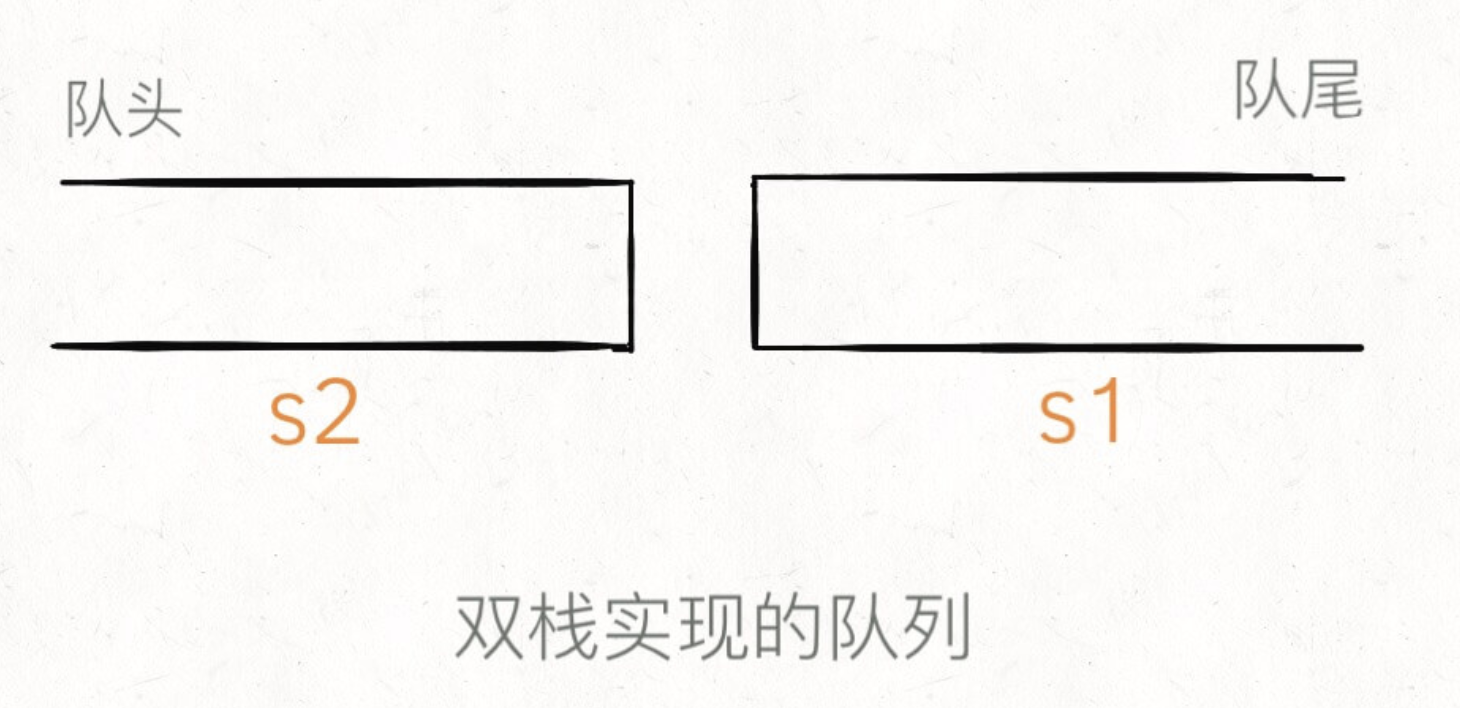
\includegraphics[width=.5\textwidth]{fig/Queue_Stack_Implementation_1.png}
\end{figure}

\begin{lstlisting}
class MyQueue {
    private Stack<Integer> s1, s2;
    
    public MyQueue() {
        s1 = new Stack<>();
        s2 = new Stack<>();
    }
    // ...
}
\end{lstlisting}

当调用 push 让元素入队时,只要把元素压入 s1 即可,比如说 push 进 3 个元素分别是 1,2,3,那么底层结构就是这样:
\begin{figure}[H]
    \centering
    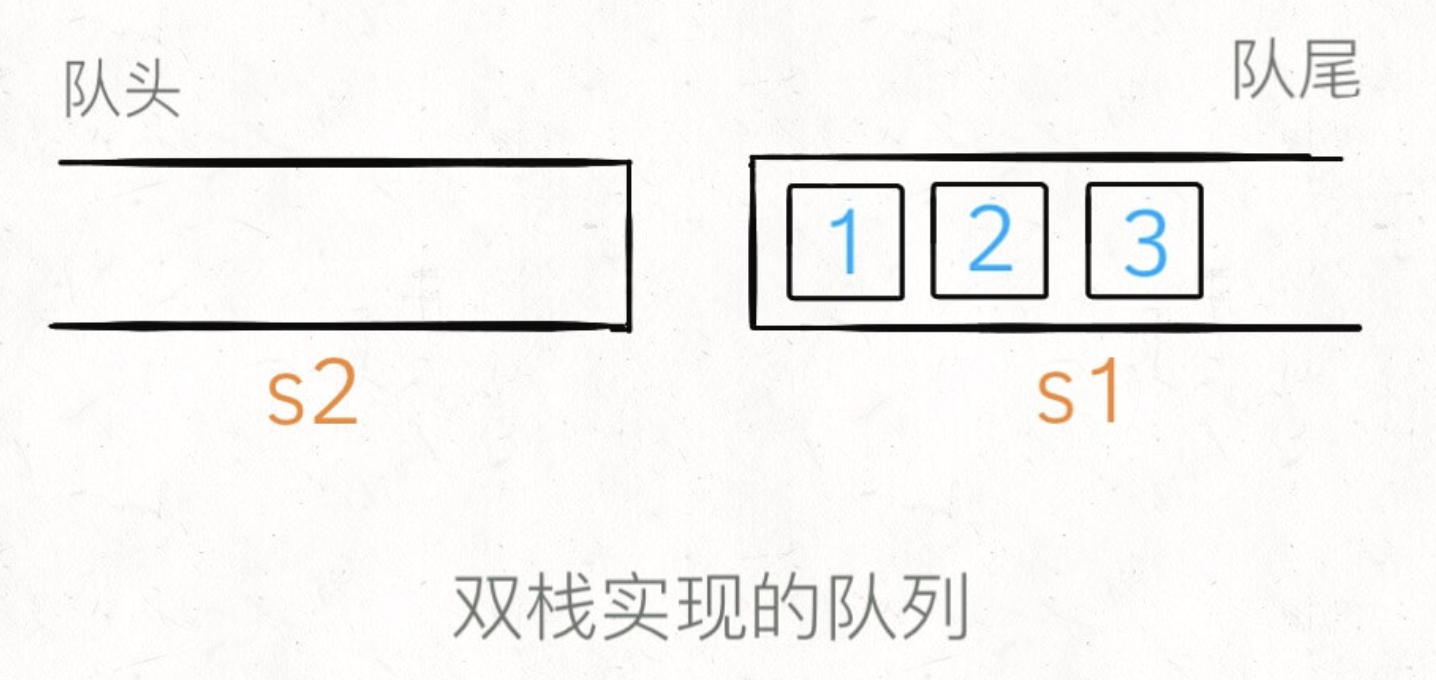
\includegraphics[width=.5\textwidth]{fig/Queue_Stack_Implementation_2.png}
\end{figure}

\begin{lstlisting}
/** 添加元素到队尾 */
public void push(int x) {
    s1.push(x);
}
\end{lstlisting}

那么如果这时候使用 peek 查看队头的元素怎么办呢?按道理队头元素应该是 1,但是在 s1 中 1 被压在栈底,现在就要轮到 s2 起到一个中转的作用了:当 s2 为空时,可以把 s1 的所有元素取出再添加进 s2,\textbf{这时候 s2 中元素就是先进先出顺序了}。
\begin{figure}[H]
    \centering
    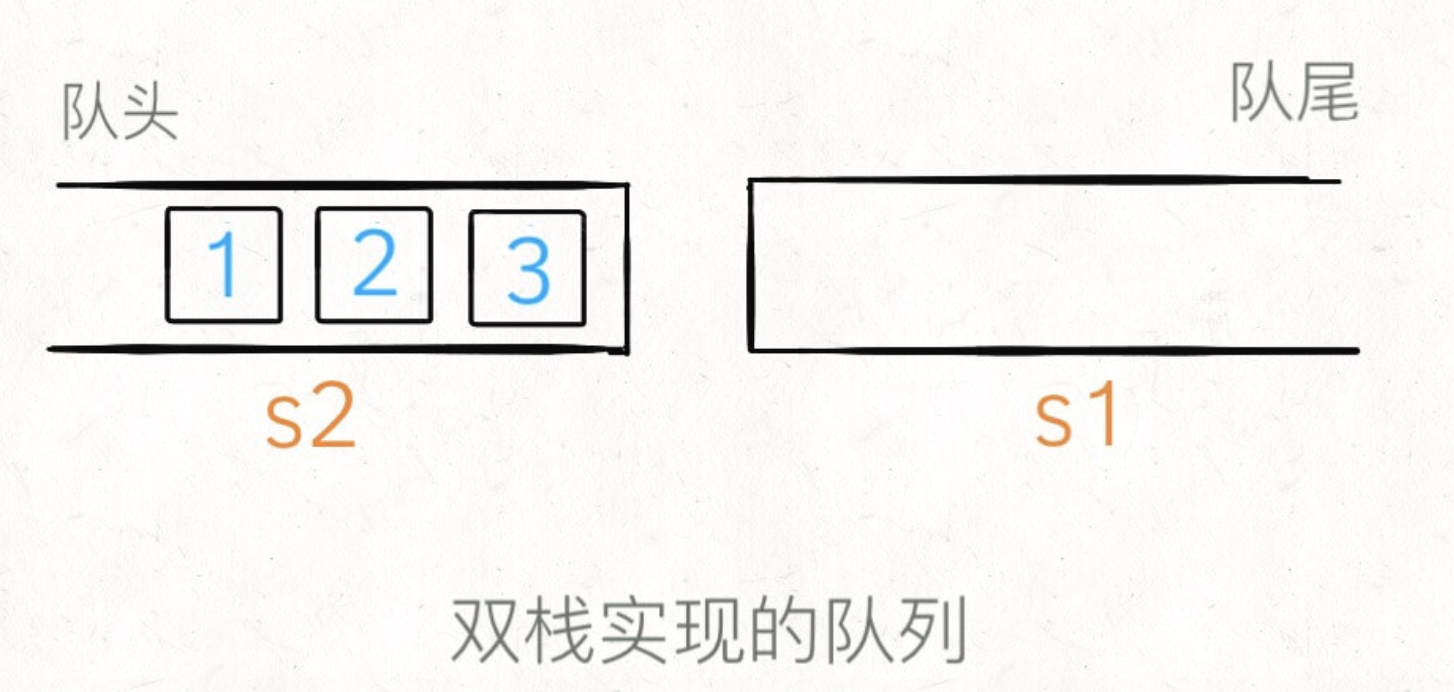
\includegraphics[width=.5\textwidth]{fig/Queue_Stack_Implementation_3.png}
\end{figure}

\begin{lstlisting}
/** 返回队头元素 */
public int peek() {
    if (s2.isEmpty())
        // 把 s1 元素压入 s2
        while (!s1.isEmpty())
            s2.push(s1.pop());
    return s2.peek();
}
\end{lstlisting}

同理,对于 pop 操作,只要操作 s2 就可以了。
\begin{lstlisting}
/** 删除队头的元素并返回 */
public int pop() {
    // 先调用 peek 保证 s2 非空
    peek();
    return s2.pop();
}
\end{lstlisting}

最后,如何判断队列是否为空呢?如果两个栈都为空的话,就说明队列为空:
\begin{lstlisting}
/** 判断队列是否为空 */
public boolean empty() {
    return s1.isEmpty() && s2.isEmpty();
}
\end{lstlisting}

至此,就用栈结构实现了一个队列,核心思想是利用两个栈互相配合。

值得一提的是,这几个操作的时间复杂度是多少呢?有点意思的是 peek 操作,调用它时可能触发 while 循环,这样的话时间复杂度是 O(N),但是大部分情况下 while 循环不会被触发,时间复杂度是 O(1)。由于 pop 操作调用了 peek,它的时间复杂度和 peek 相同。

像这种情况,可以说它们的最坏时间复杂度是 O(N),因为包含 while 循环,可能需要从 s1 往 s2 搬移元素。

但是它们的均摊时间复杂度是 O(1),这个要这么理解:对于一个元素,最多只可能被搬运一次,也就是说 peek 操作平均到每个元素的时间复杂度是 O(1)。

\subsection{用队列实现栈}
如果说双栈实现队列比较巧妙,那么用队列实现栈就比较简单粗暴了,只需要一个队列作为底层数据结构。首先看下栈的 API:
\begin{lstlisting}
class MyStack {
    
    /** 添加元素到栈顶 */
    public void push(int x);
    
    /** 删除栈顶的元素并返回 */
    public int pop();
    
    /** 返回栈顶元素 */
    public int top();
    
    /** 判断栈是否为空 */
    public boolean empty();
}
\end{lstlisting}

先说 push API,直接将元素加入队列,同时记录队尾元素,因为队尾元素相当于栈顶元素,如果要 top 查看栈顶元素的话可以直接返回:
\begin{lstlisting}
class MyStack {
    Queue<Integer> q = new LinkedList<>();
    int top_elem = 0;

    /** 添加元素到栈顶 */
    public void push(int x) {
        // x 是队列的队尾,是栈的栈顶
        q.offer(x);
        top_elem = x;
    }
    
    /** 返回栈顶元素 */
    public int top() {
        return top_elem;
    }
}
\end{lstlisting}

我们的底层数据结构是先进先出的队列,每次 pop 只能从队头取元素;但是栈是后进先出,也就是说 pop API 要从队尾取元素。
\begin{figure}[H]
    \centering
    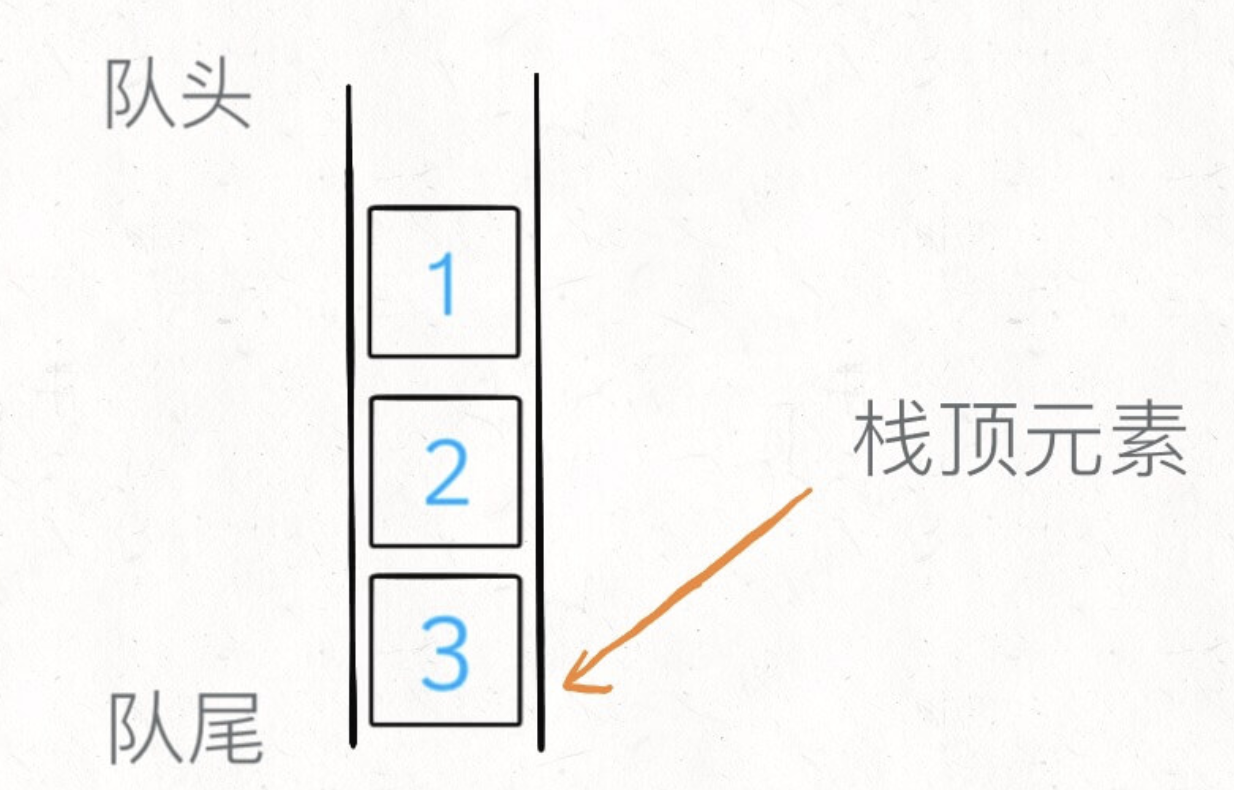
\includegraphics[width=.5\textwidth]{fig/Queue_Stack_Implementation_4.png}
\end{figure}

解决方法简单粗暴,把队列前面的都取出来再加入队尾,让之前的队尾元素排到队头,这样就可以取出了:
\begin{figure}[H]
    \centering
    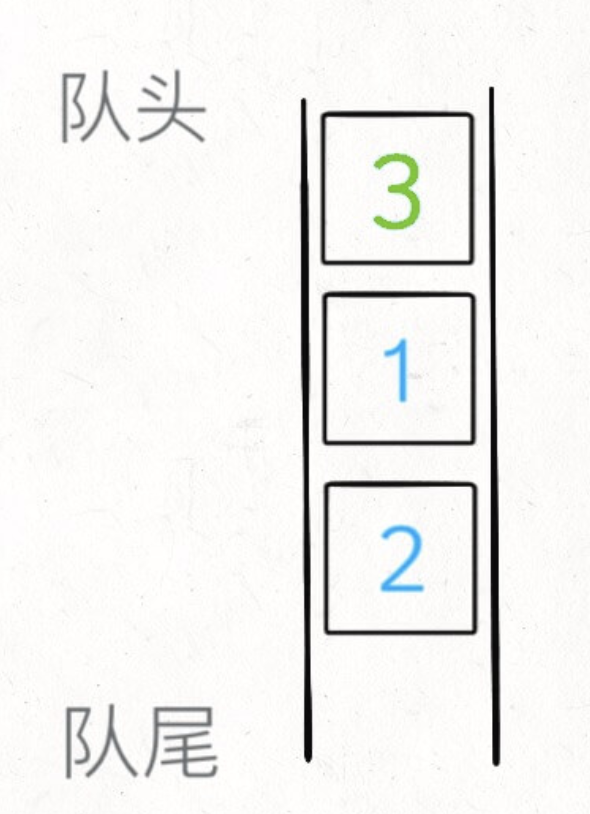
\includegraphics[width=.3\textwidth]{fig/Queue_Stack_Implementation_5.png}
\end{figure}

\begin{lstlisting}
/** 删除栈顶的元素并返回 */
public int pop() {
    int size = q.size();
    while (size > 1) {
        q.offer(q.poll());
        size--;
    }
    // 之前的队尾元素已经到了队头
    return q.poll();
}
\end{lstlisting}

这样实现还有一点小问题就是,原来的队尾元素被提到队头并删除了,但是 top\_elem 变量没有更新,我们还需要一点小修改:
\begin{lstlisting}
/** 删除栈顶的元素并返回 */
public int pop() {
    int size = q.size();
    // 留下队尾 2 个元素
    while (size > 2) {
        q.offer(q.poll());
        size--;
    }
    // 记录新的队尾元素
    top_elem = q.peek();
    q.offer(q.poll());
    // 删除之前的队尾元素
    return q.poll();
}
\end{lstlisting}

最后,API empty 就很容易实现了,只要看底层的队列是否为空即可:
\begin{lstlisting}
/** 判断栈是否为空 */
public boolean empty() {
    return q.isEmpty();
}
\end{lstlisting}

很明显,用队列实现栈的话,pop 操作时间复杂度是 O(N),其他操作都是 O(1)​。​

个人认为,用队列实现栈是没啥亮点的问题,但是用双栈实现队列是值得学习的。

从栈 s1 搬运元素到 s2 之后,元素在 s2 中就变成了队列的先进先出顺序,这个特性有点类似「负负得正」,确实不太容易想到。

%\printbibliography
\bibliography{../ref}
\bibliographystyle{IEEEtran}
\end{document}